\chapter{Quench Recognition Problem (QRP)}
\label{chp:qrp}
This chapter is dedicated to the solution of \qrp, which we introduced in \Cref{chp:problem}, in this chapter we will:
\begin{itemize}
	\item Give a rapid overview of the problem, analyzing the results obtained from
	      preprocessing,
	\item Talk about the models used, and the results obtained for each model,
	\item Select the 'best' possible model.
\end{itemize}

\section{Problem description}
As was introduced in the previous chapter out dataset consisted of four tables of $279$ samples
each, divided between 'quench' and 'non-quench' events, the distribution is not exactly balanced:
$192$ quench events and $87$ non-quench events; since the imbalance is not extreme we didn't take
explicit action against it.

\section{Data preprocessing}
Before working on the actual models we analyzed:
\begin{inparaenum}[(i)]
	\item the cross-correlations between the harmonics,
	\item the cross-correlation between the harmonics and the labels,
	\item the box plot of the attributes, and
	\item the distribution of data after dimensionality reduction via principal component analysis (PCA).
\end{inparaenum}.
In the following, the vector containing the information about the correlation with the labels has been plotted after a
normalization step, which was done with the MinMaxScaler class of scikit-learn. While this procedure
doesn't change the intensity of the correlation between the harmonic and the label it makes the
graphs more readable and easier to interpret, the normalized samples are scaled using
\Cref{eq:normalization} \cite{Nishok2024}.
\begin{equation}
	\label{eq:normalization}
	X_\text{scaled} = \frac{X - X_\text{min}}{X_\text{max} - X_\text{min}}
\end{equation}
Where $X$ is a sample in the vector that is being scaled.

The results are reported in the following sections, one for each table.

\subsubsection{\an\ table}
\Cref{fig:an-corr} shows the correlation of the various harmonics with each other. Independently
of the sign of the cross-correlation measurement, there is a clear pattern contained in the matrix,
indicating that many harmonics contain repeated information, e.g., harmonic number $1$ provides the same information as harmonic number $3, 5, 7, \ldots$.
\begin{figure}
	\centering
	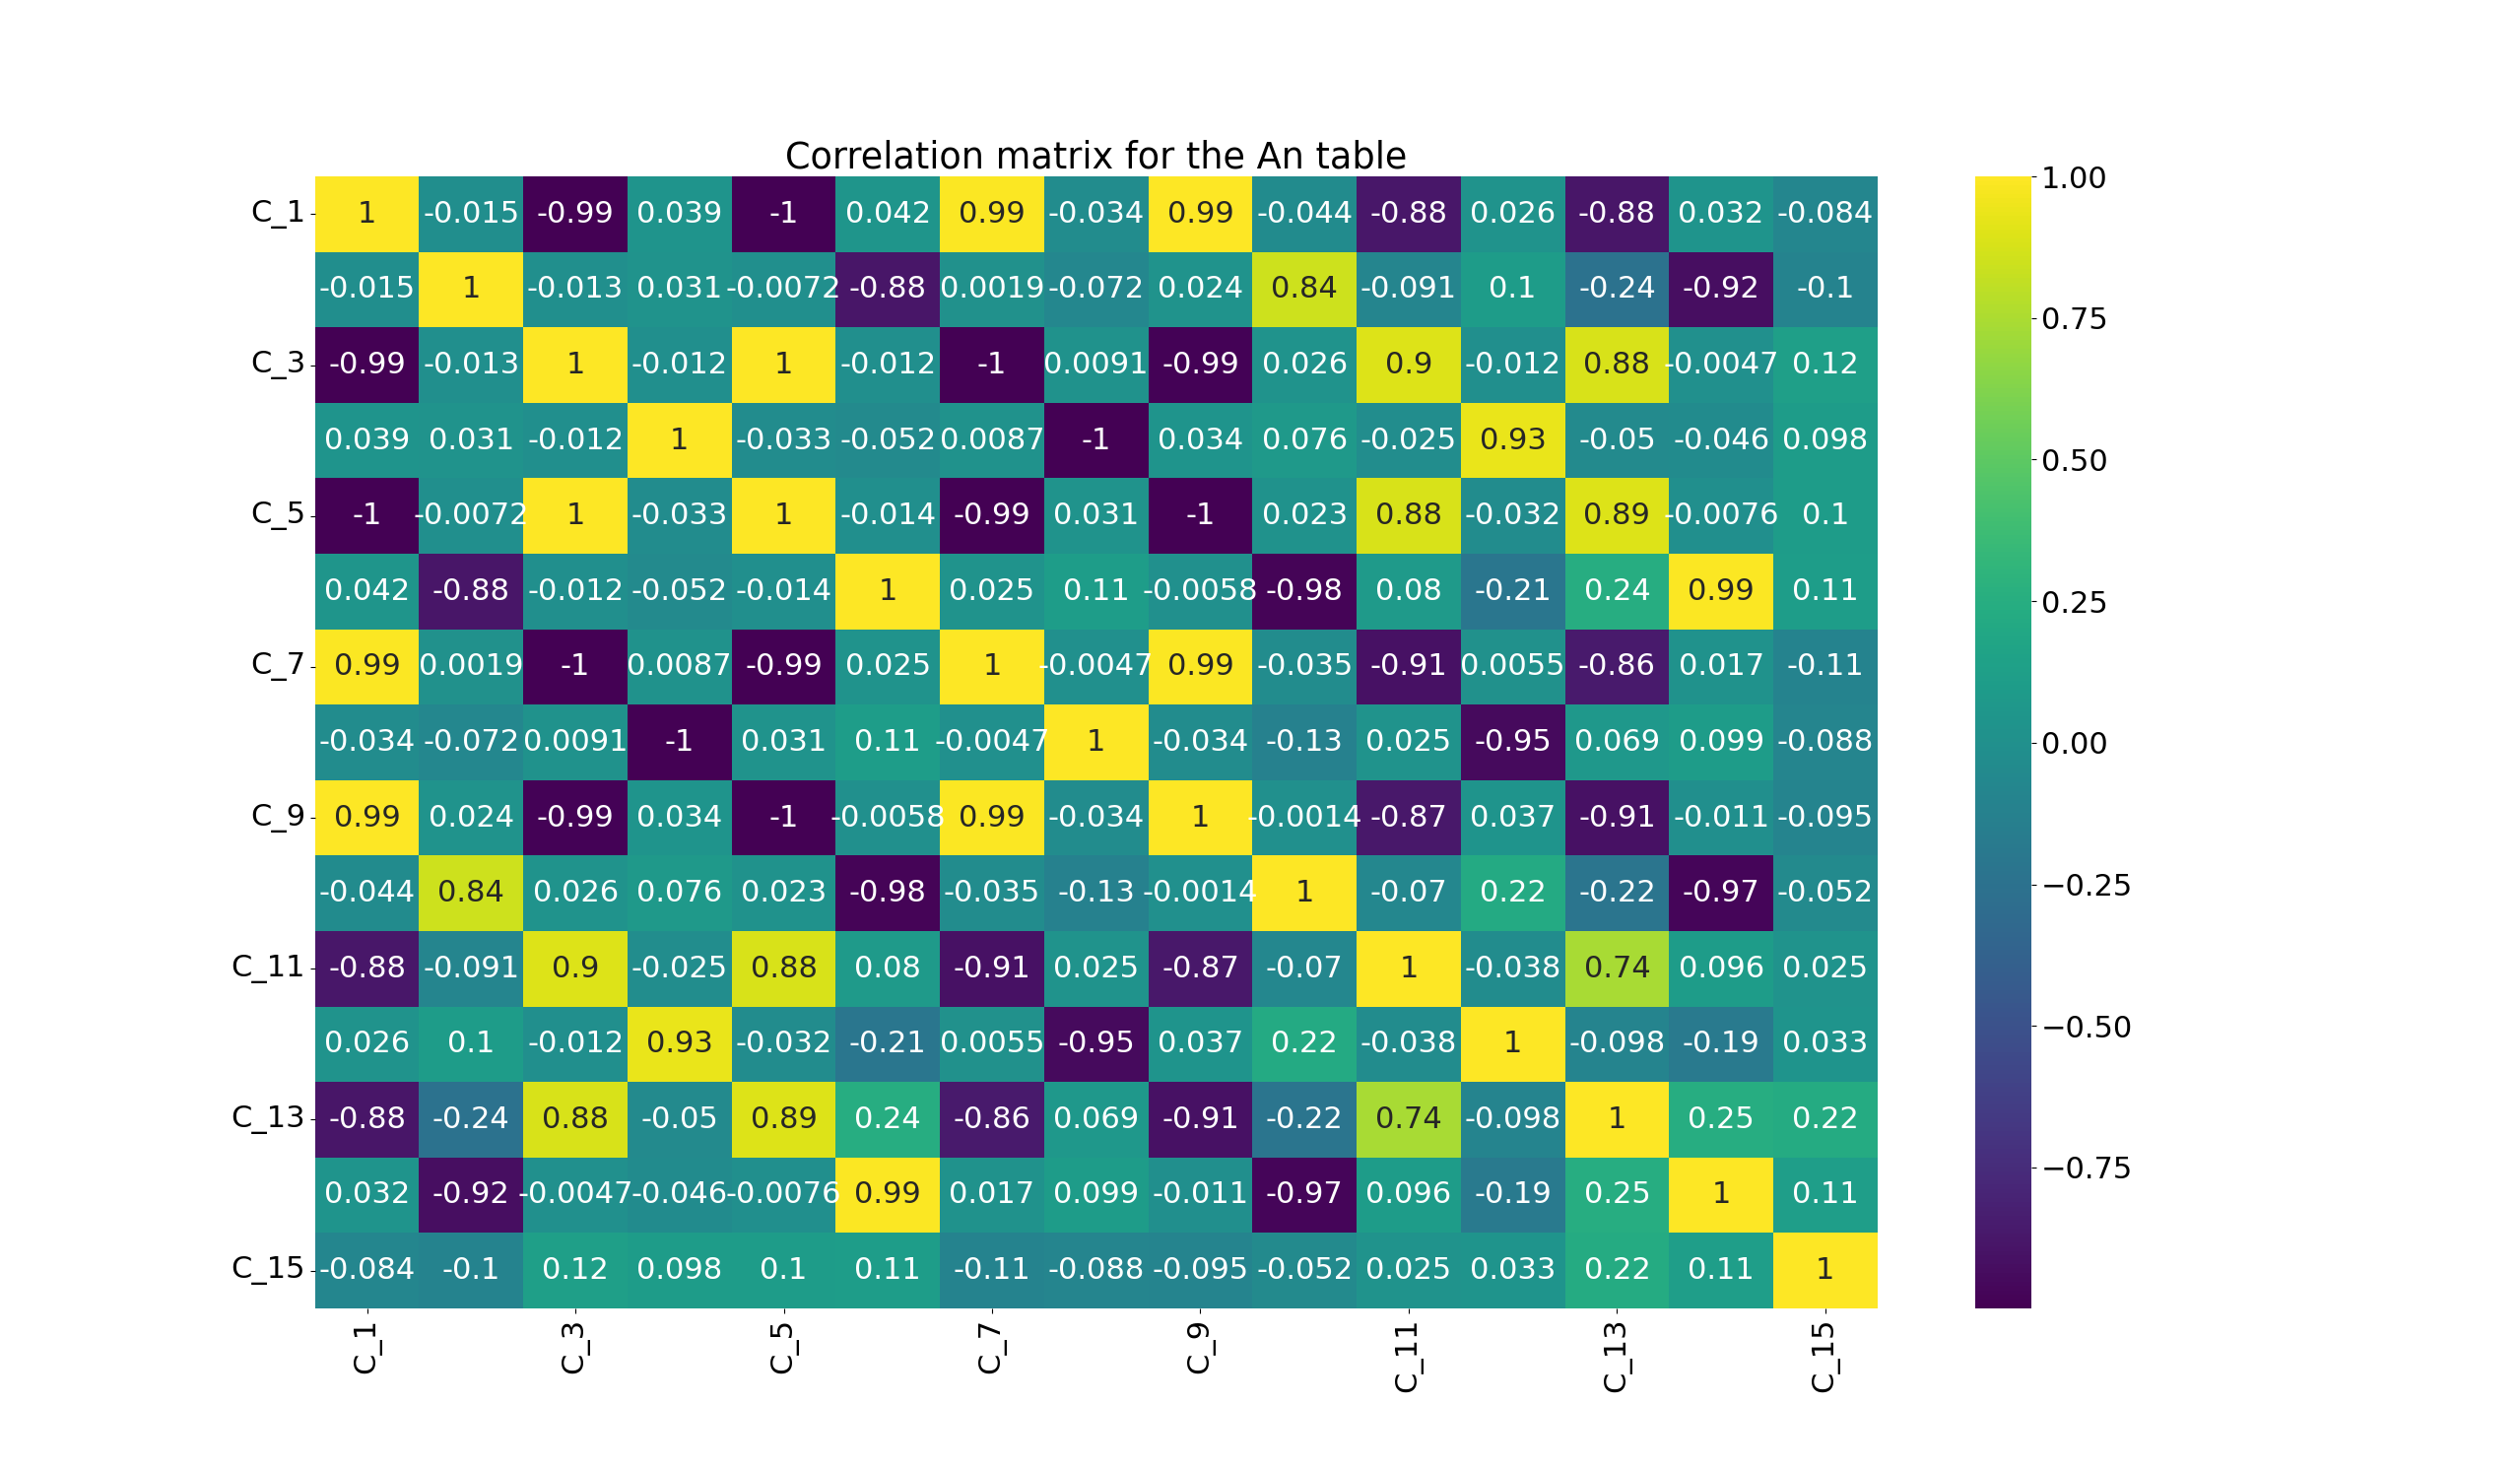
\includegraphics[width=\linewidth]{img/An_corr_matrix.png}
	\caption{The cross-correlation of the \an\ harmonics} \label{fig:an-corr}
\end{figure}

By looking at \Cref{fig:an-corr} we can gather the following information:
\begin{itemize}
	\item Its strong geometry implies that doing feature extraction is going to be complex, due to the necessity of finding a mix of harmonics that has a high correlation with the label, while having a low correlation among themselves.
	\item All the odd harmonics are strongly correlated with each other (with the sole exception
	      of harmonic $15$),
	\item Harmonic number $2$ is strongly correlated with its odd multiples,
	\item Harmonic number $4$ is strongly correlated with all its multiples,
	\item Harmonic number $15$ is the only one that is not correlated to any of the other
	      harmonics.
\end{itemize}

\Cref{fig:an-lcorr} aims to show how informative the various harmonics with regard to the single
label ('quench' or 'non-quench').

\begin{figure}
	\centering
	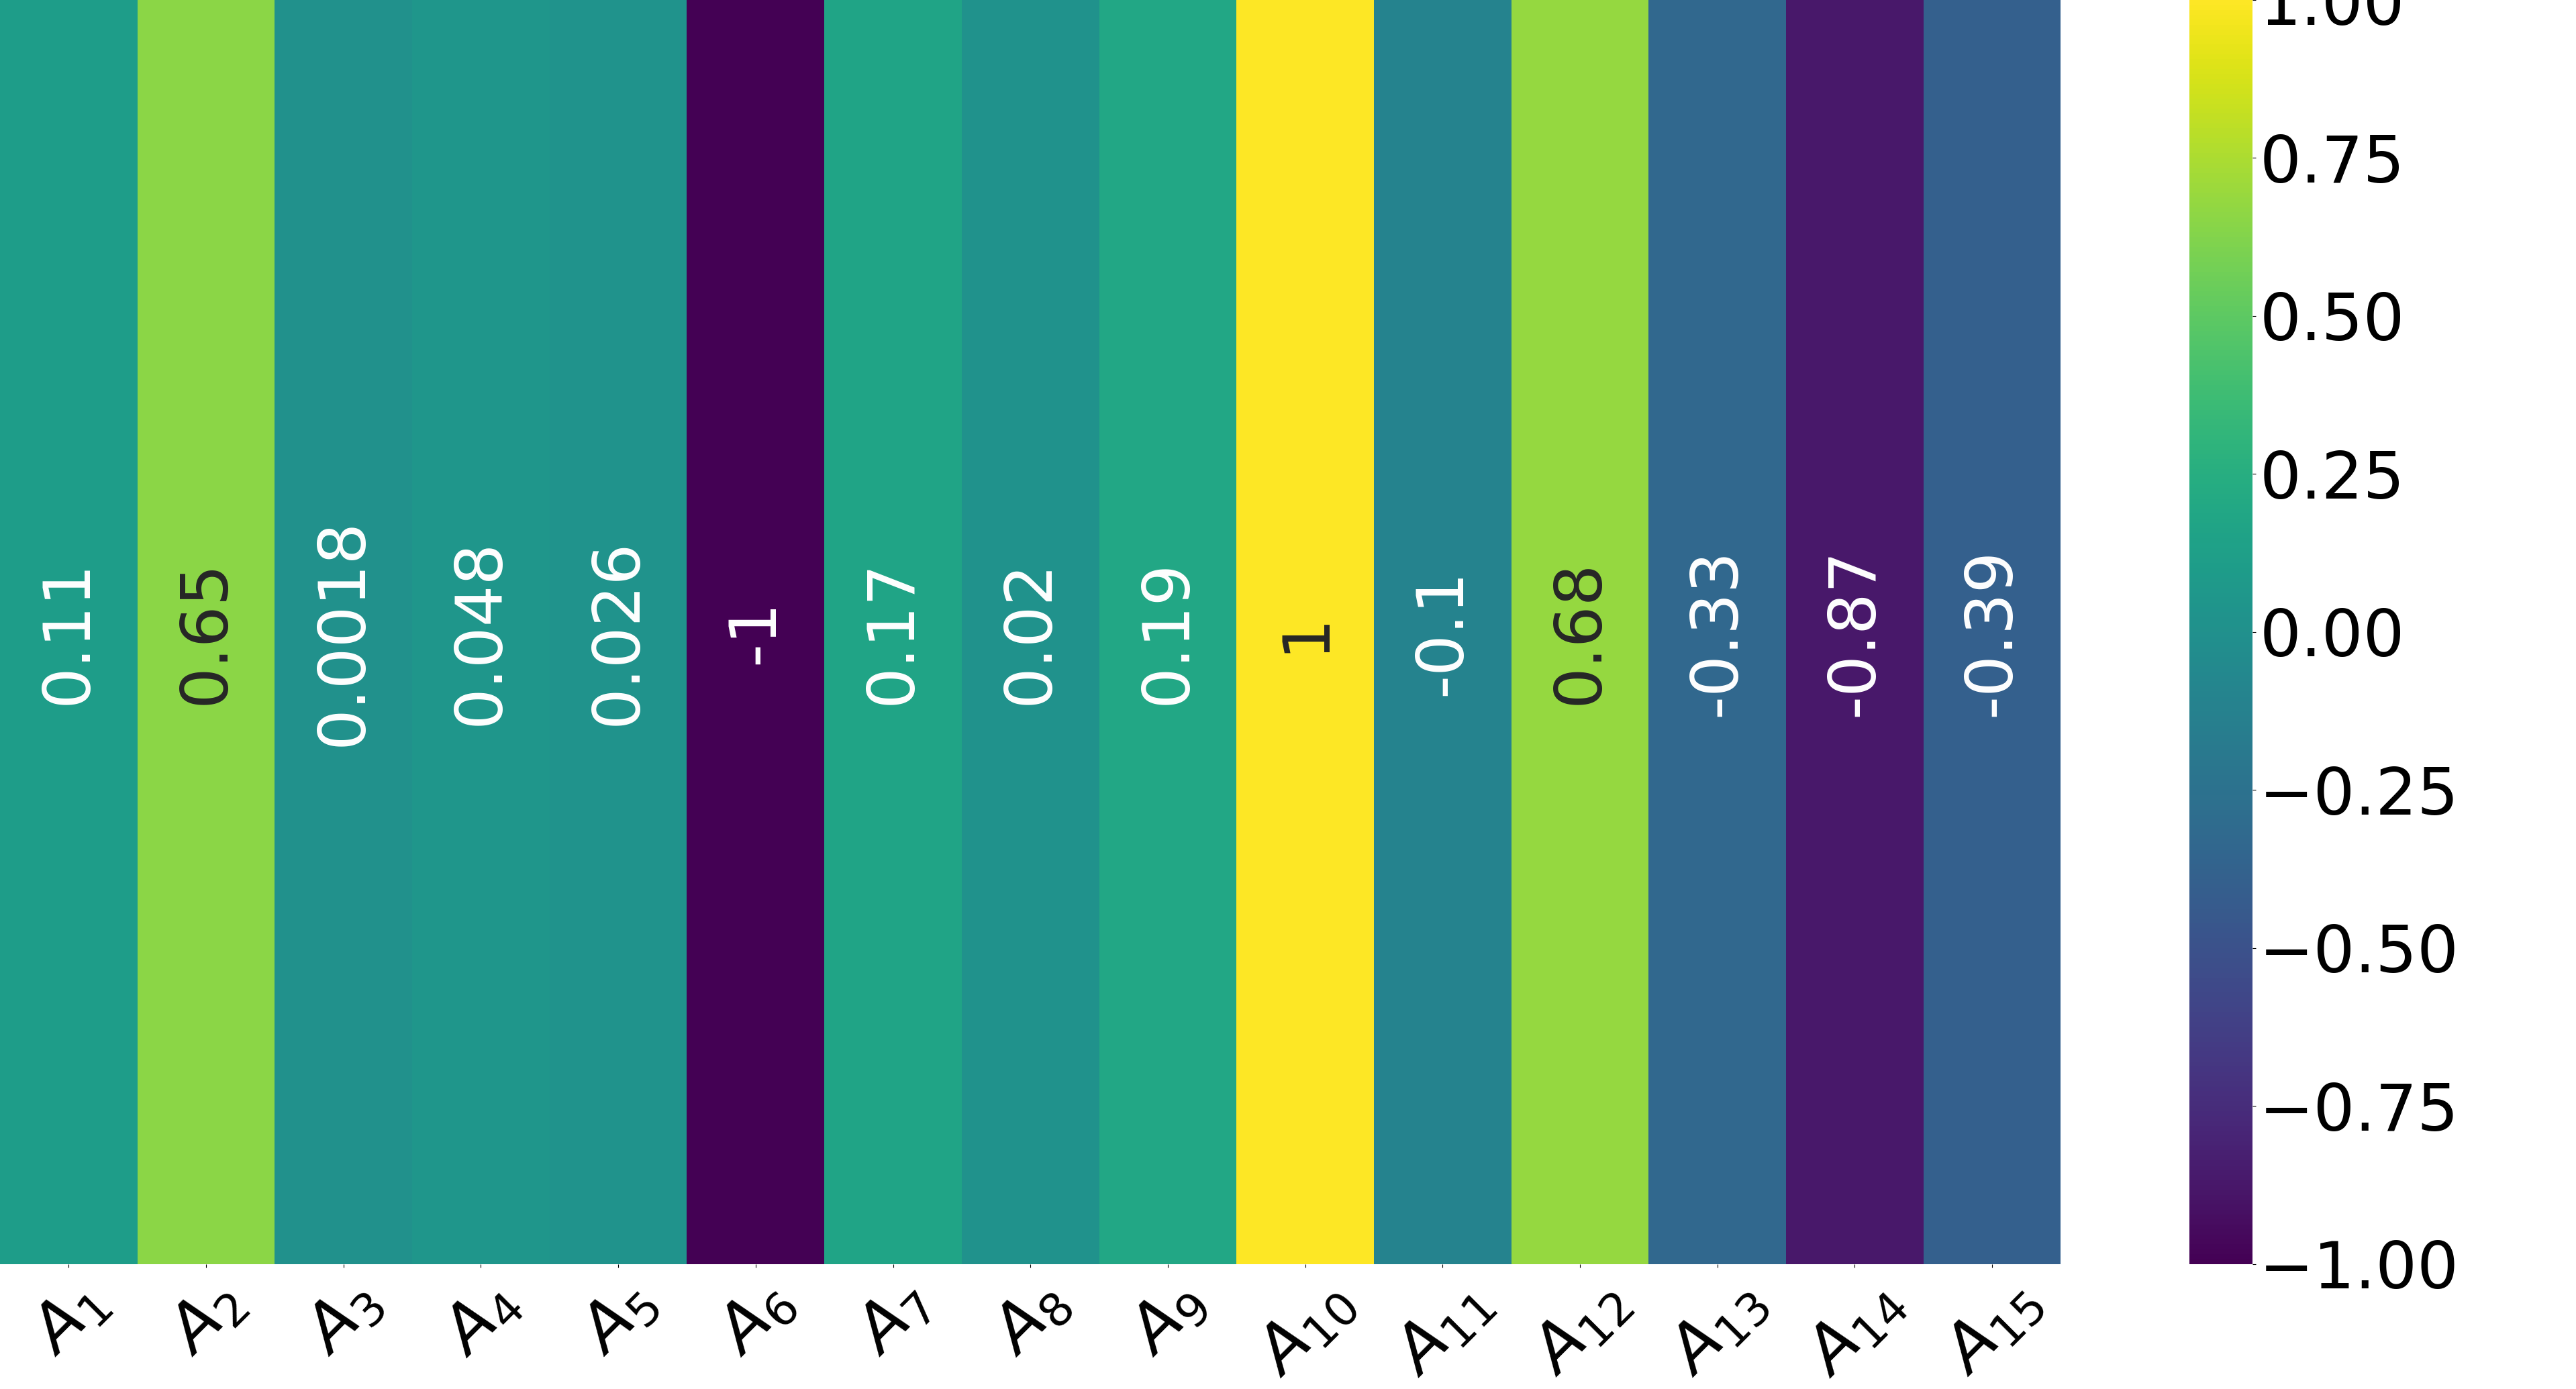
\includegraphics[width=\linewidth]{img/An_label_corr.png}
	\caption{Label correlation for the \an\ table} \label{fig:an-lcorr}
\end{figure}

Once again, considering \Cref{fig:an-lcorr}, we picked the harmonics with the highest label
correlation, which are identified by a higher color intensity; as we can see the label is explained
very well by harmonics number: $2, 6, 10, 11, 12, 13, 14, 15$.
These conclusions are doubly interesting, since:
\begin{enumerate}
	\item The $2^{nd}$ harmonic, as well as its odd multiples, can explain the results well, which
	      is what we expect from the theory.
	\item High order harmonics are able to explain the results better than other harmonics,
	      which is not what we would have expect, since in the original analysis the value for the
	      labels was computed using primarily lower order harmonics.
\end{enumerate}

Based on all the information obtained up to this point we can conjecture that some of the best
datasets will probably contain the second harmonic, or one of its high order odd multiples, as well
as harmonic number $15$, and some other high order harmonic (i.e.: harmonics number $11$ or $13$). As we will see
in the following one of the best datasets that we built on this table was based on harmonics $2, 12$.

Lastly, we can visualize the distribution of the samples in bidimensional space, which was achieved
by using a dimensionality reduction technique, namely $\textsc{pca}$ (Principal Component Analysis).
\begin{figure}[h!]
	\centering
	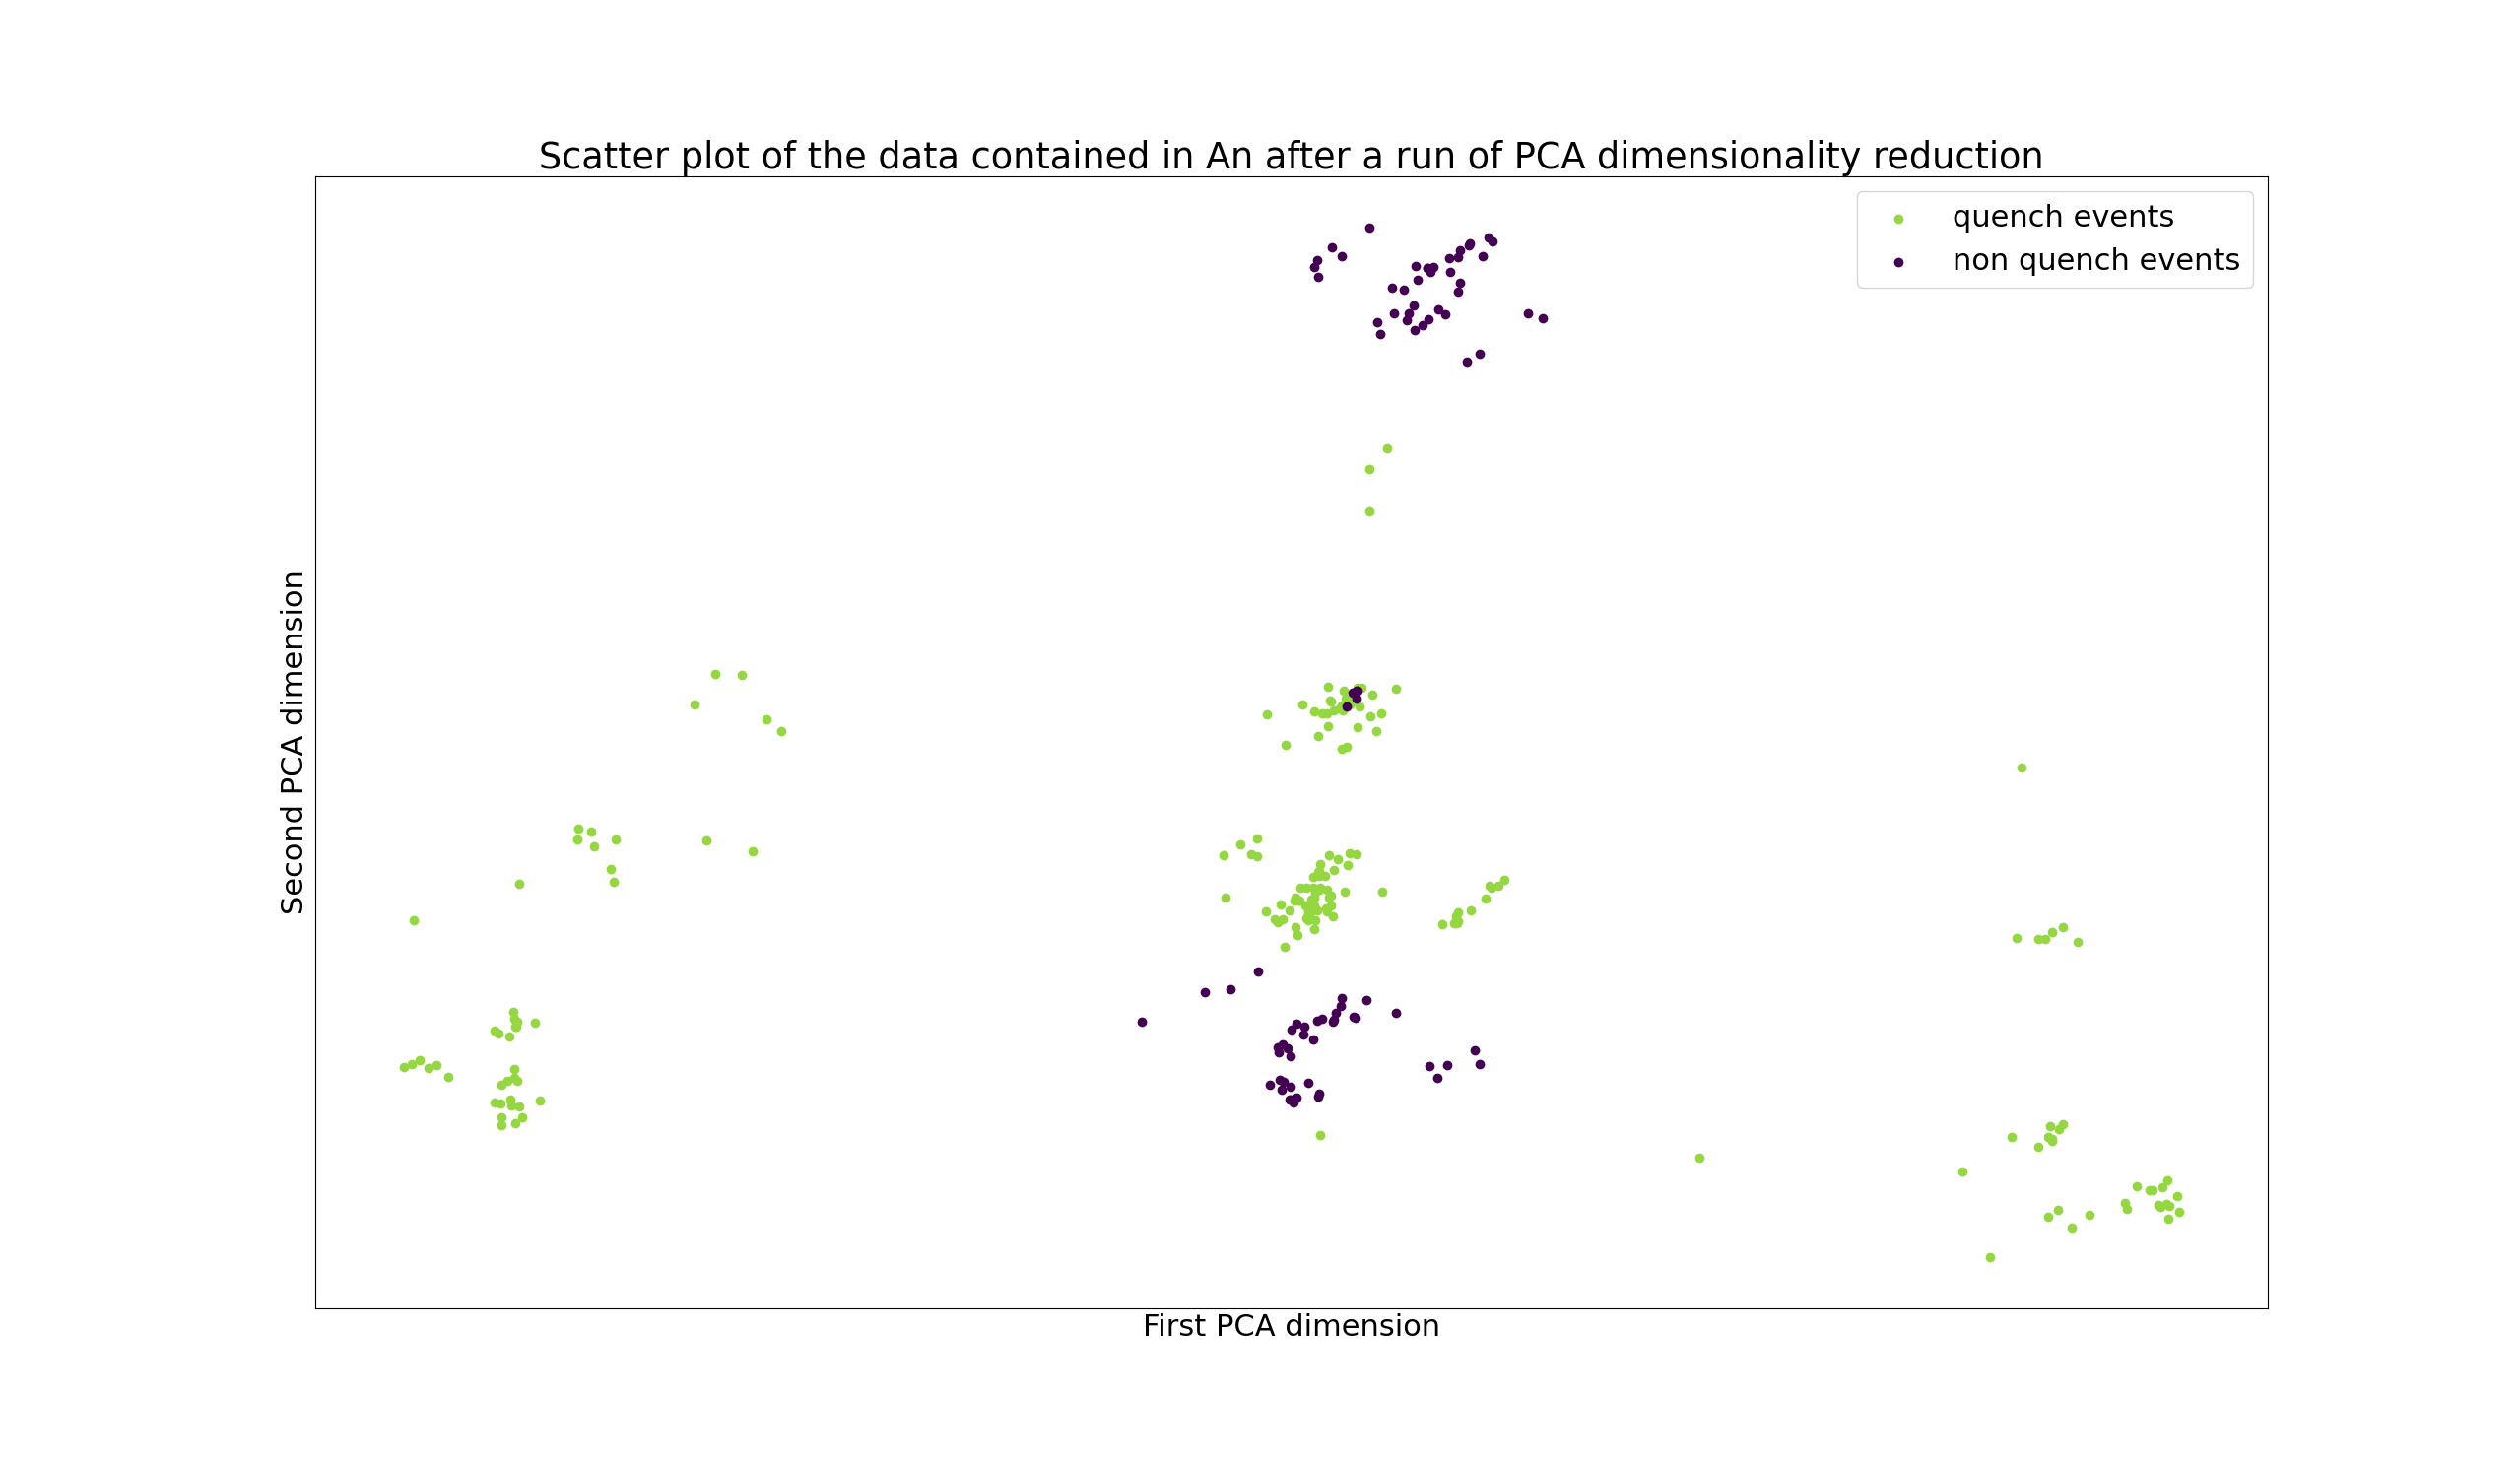
\includegraphics[width=\linewidth]{img/An_distribution.png}
	\caption{Data distribution for the \an\ table after applying $\textsc{pca}$ dimensionality
		reduction} \label{fig:an-dist}
\end{figure}

It can be seen in \Cref{fig:an-dist} that the samples, after dimensionality reduction, are distributed very nicely in a series
of zones, each zone has a very high degree of purity; this lead us to suppose that it might be the
reason why models built on \an\ and \cnmod\ perform better than the alternatives.

\subsubsection{\bn\ table}
We can use a similar procedure on the \bn\ table, which in most tests proved to be the
least-performing table. This is probably due to the poor distribution of the data, as we can see in
\Cref{fig:bn-dist}, it's really hard to find a way to separate the central portion of the samples.
\begin{figure}[h!]
	\centering
	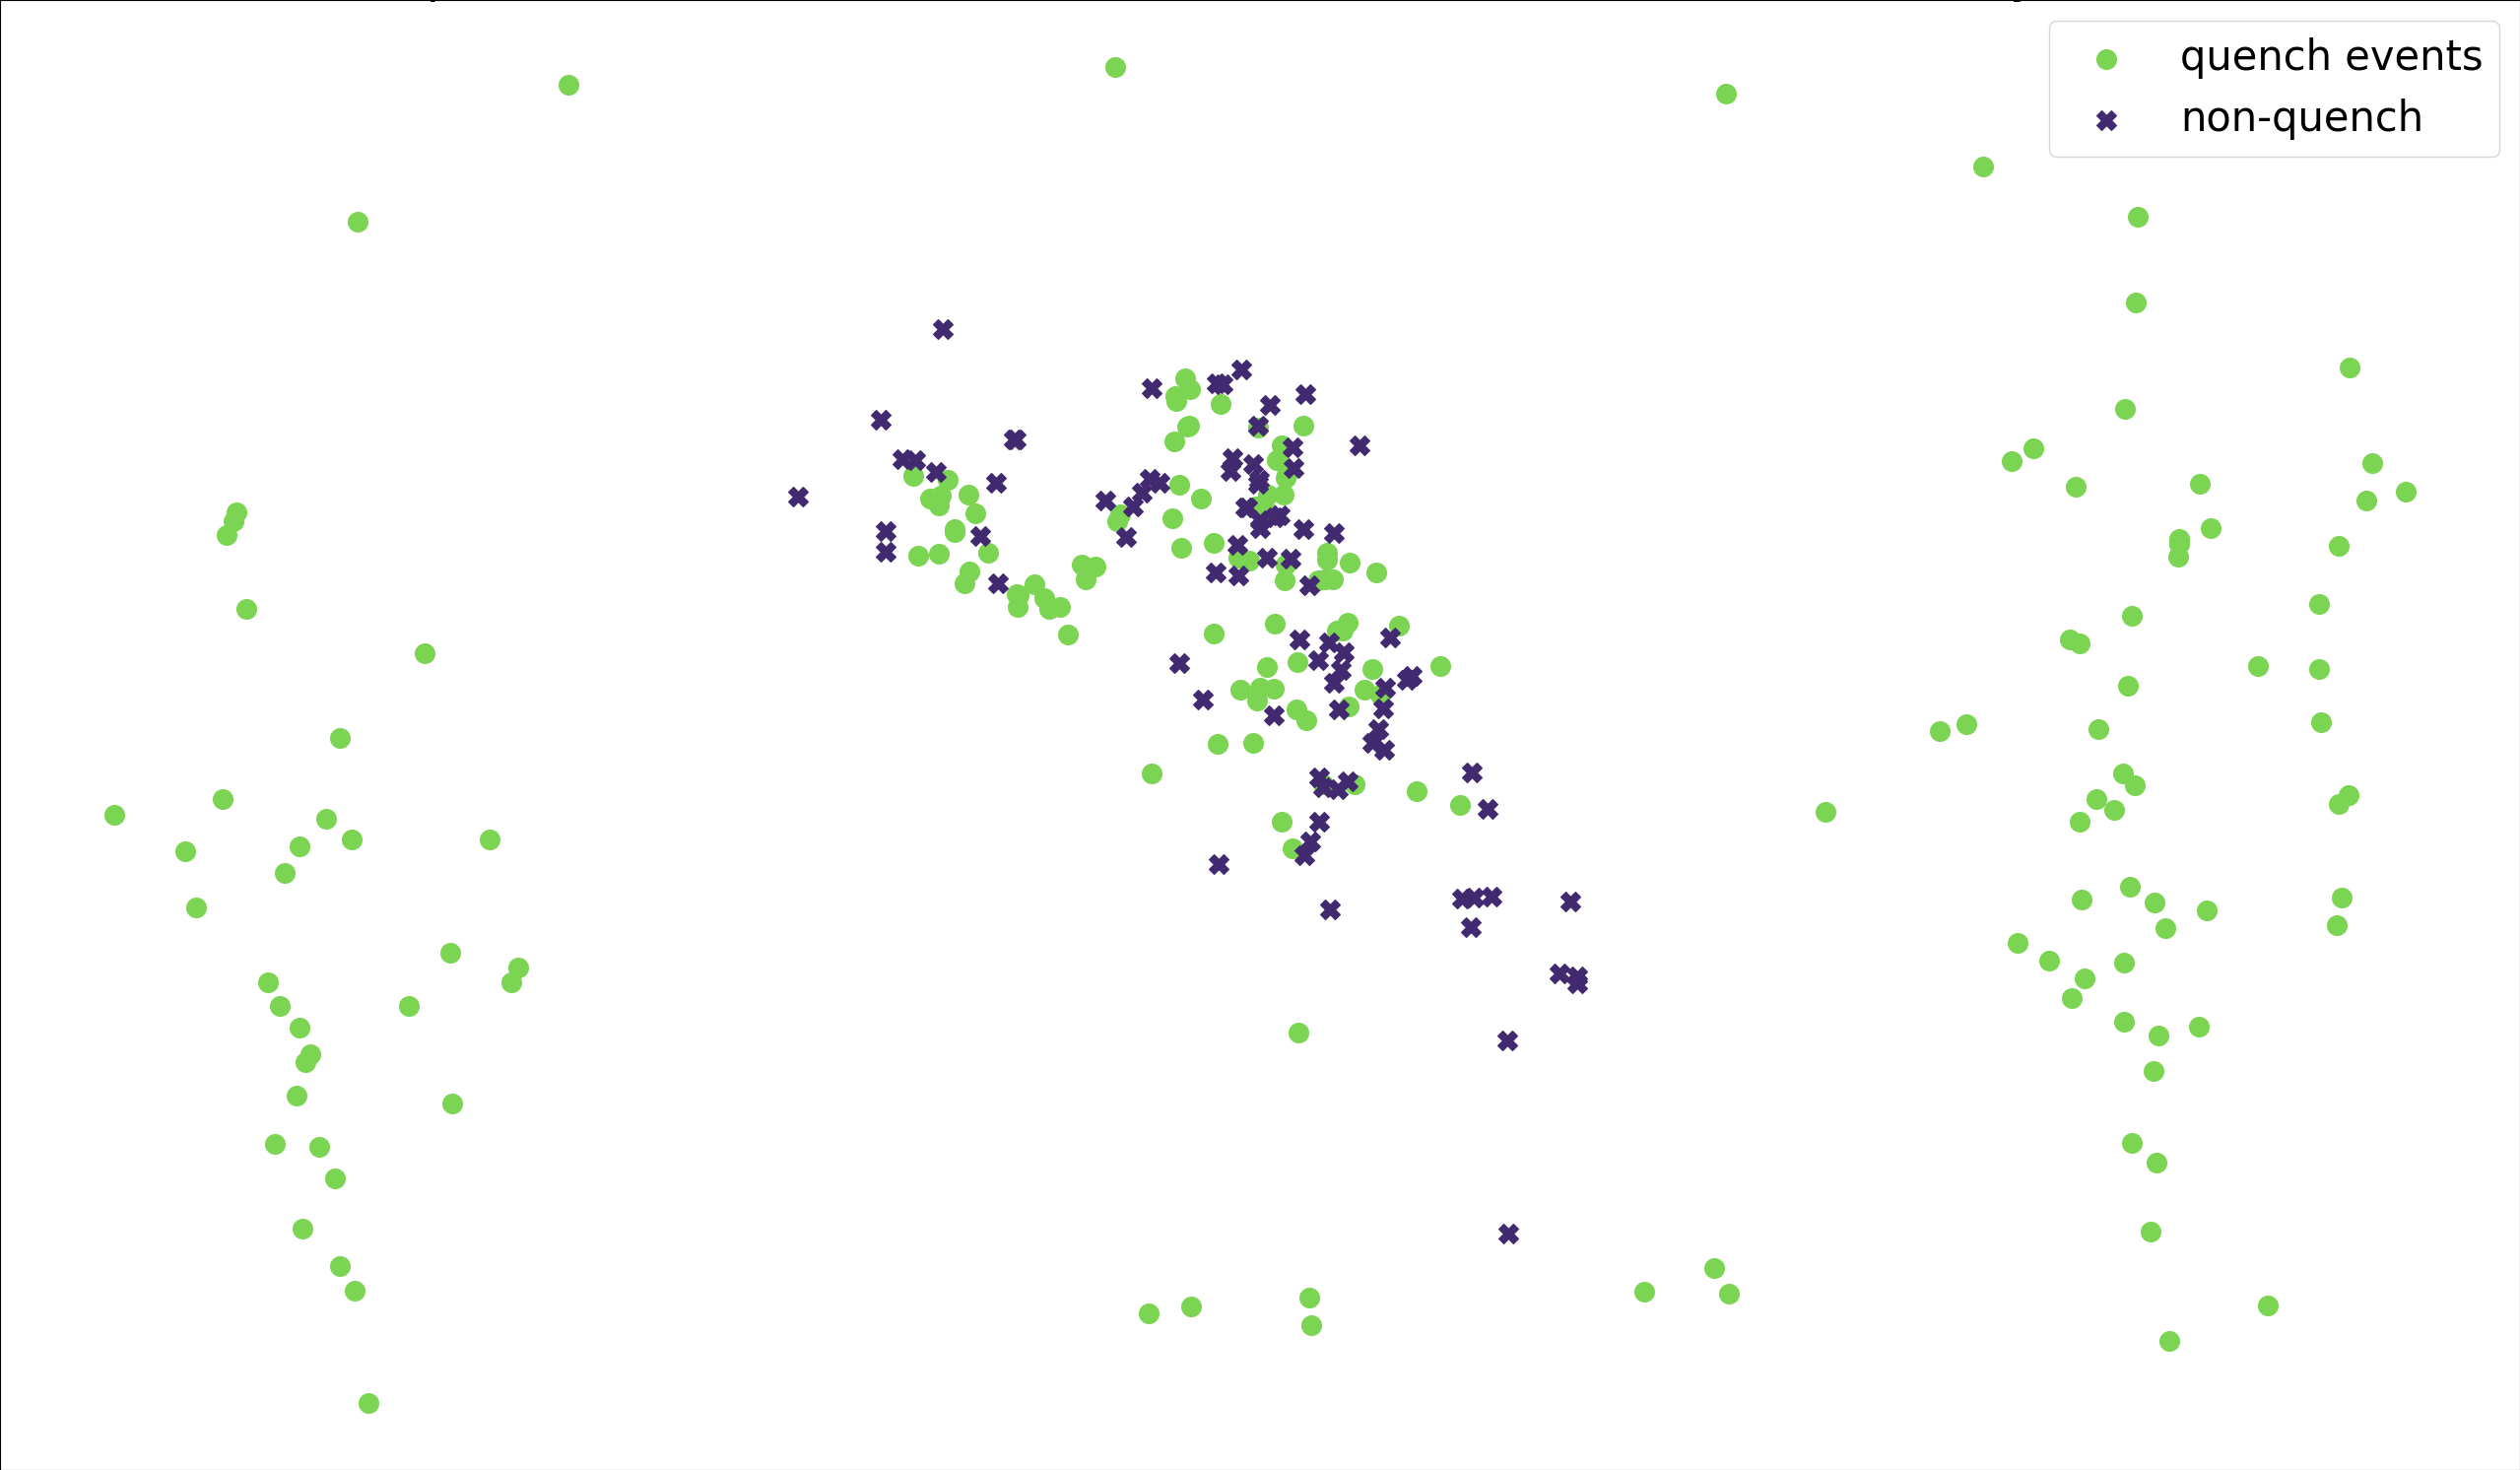
\includegraphics[width=\linewidth]{img/Bn_distribution.png}
	\caption{Data distribution for the \bn\ table after applying $\textsc{pca}$ dimensionality
		reduction} \label{fig:bn-dist}
\end{figure}

As we did for \an\ we checked the cross-correlation of the \bn\ table, and the results were actually very
similar.
\begin{figure}[h!]
	\centering
	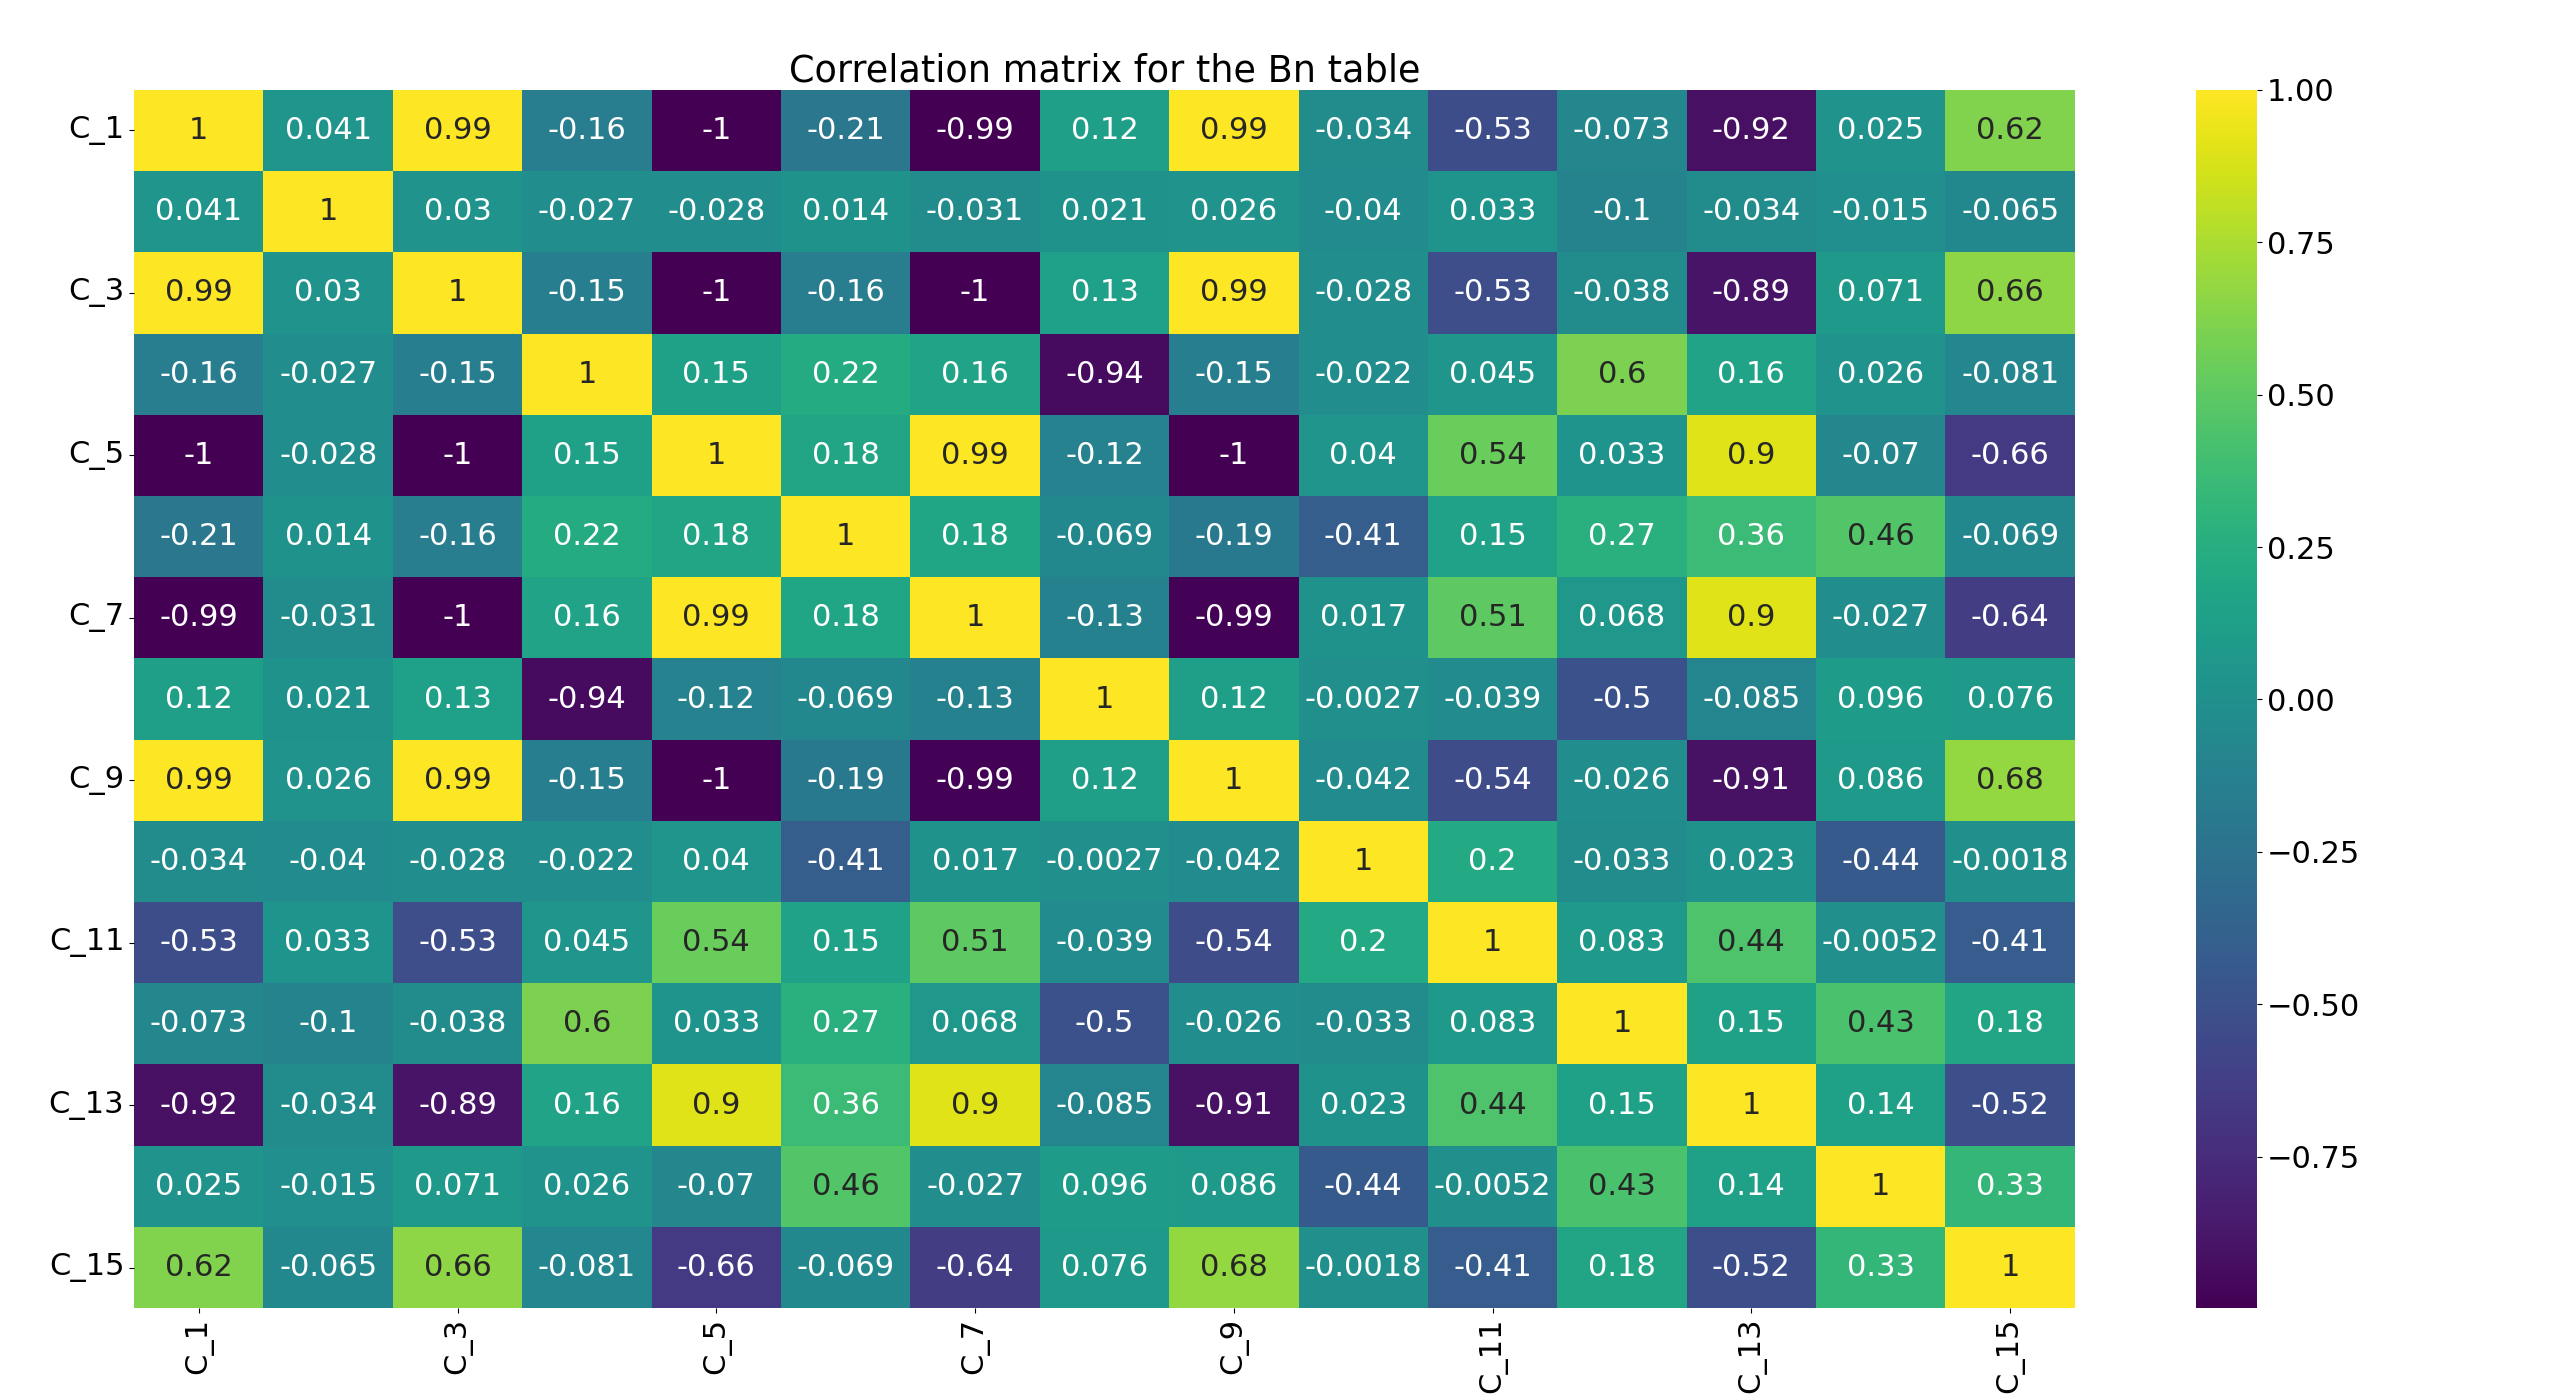
\includegraphics[width=\linewidth]{img/Bn_corr_matrix.png}
	\caption{The cross-correlation of the \bn\ harmonics} \label{fig:bn-corr}
\end{figure}
Possibly the biggest difference between \Cref{fig:an-corr} and \Cref{fig:bn-corr}, apart from the
obvious difference in the correlation values, is that harmonic $2$ is not strongly correlated with
any other harmonic, while harmonic number $15$ grows a discrete correlation with all odd harmonics.

If we check the correlation of the harmonics with the labels in (\Cref{fig:bn-lcorr}), we can see
that, apparently, most harmonics have a good enough correlation with the solution, but despite this, the performance of all
models built on \bn\ suffered.
\begin{figure}
	\centering
	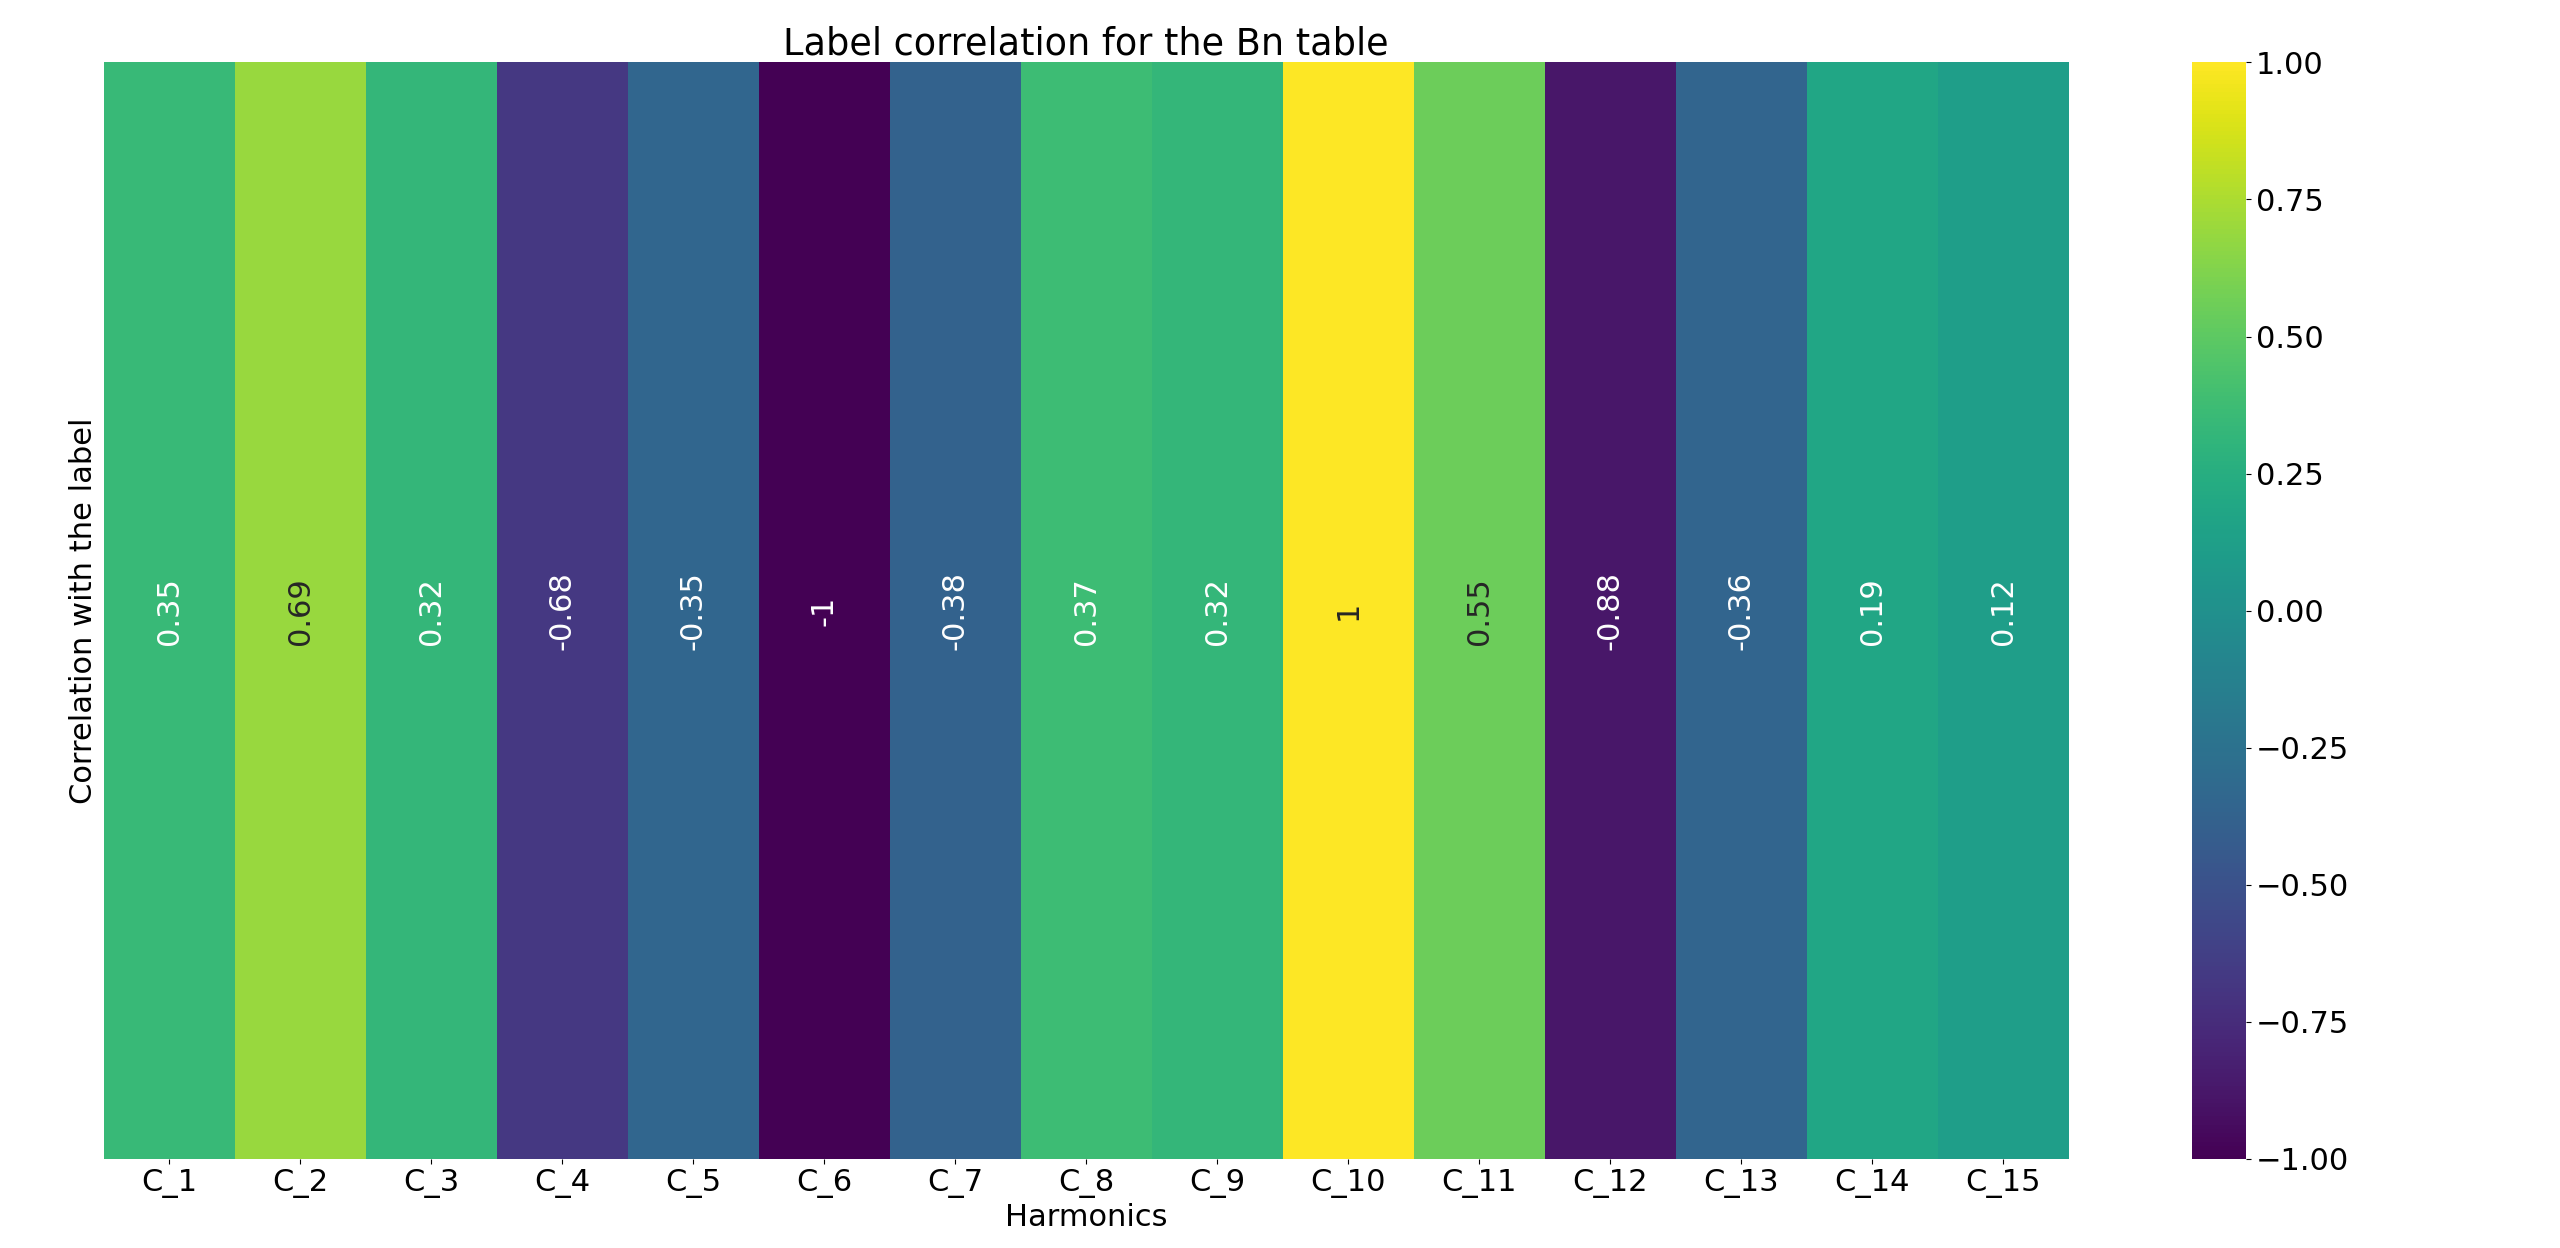
\includegraphics[width=\linewidth]{img/Bn_label_corr.png}
	\caption{Label correlation for the \bn\ table} \label{fig:bn-lcorr}
\end{figure}

\subsubsection{\cnmod\ table}
The \cnmod\ table combines the information present in \an\ and \bn, as we saw in \Cref{sec:dsets},
\cnmod\ was expected to be one of the best tables to solve \qrp, but, as we will see in future
sections, it consistently falls short of the \an\ table, probably due to the introduction of the information carried by \bn.
\begin{figure}[h!]
	\centering
	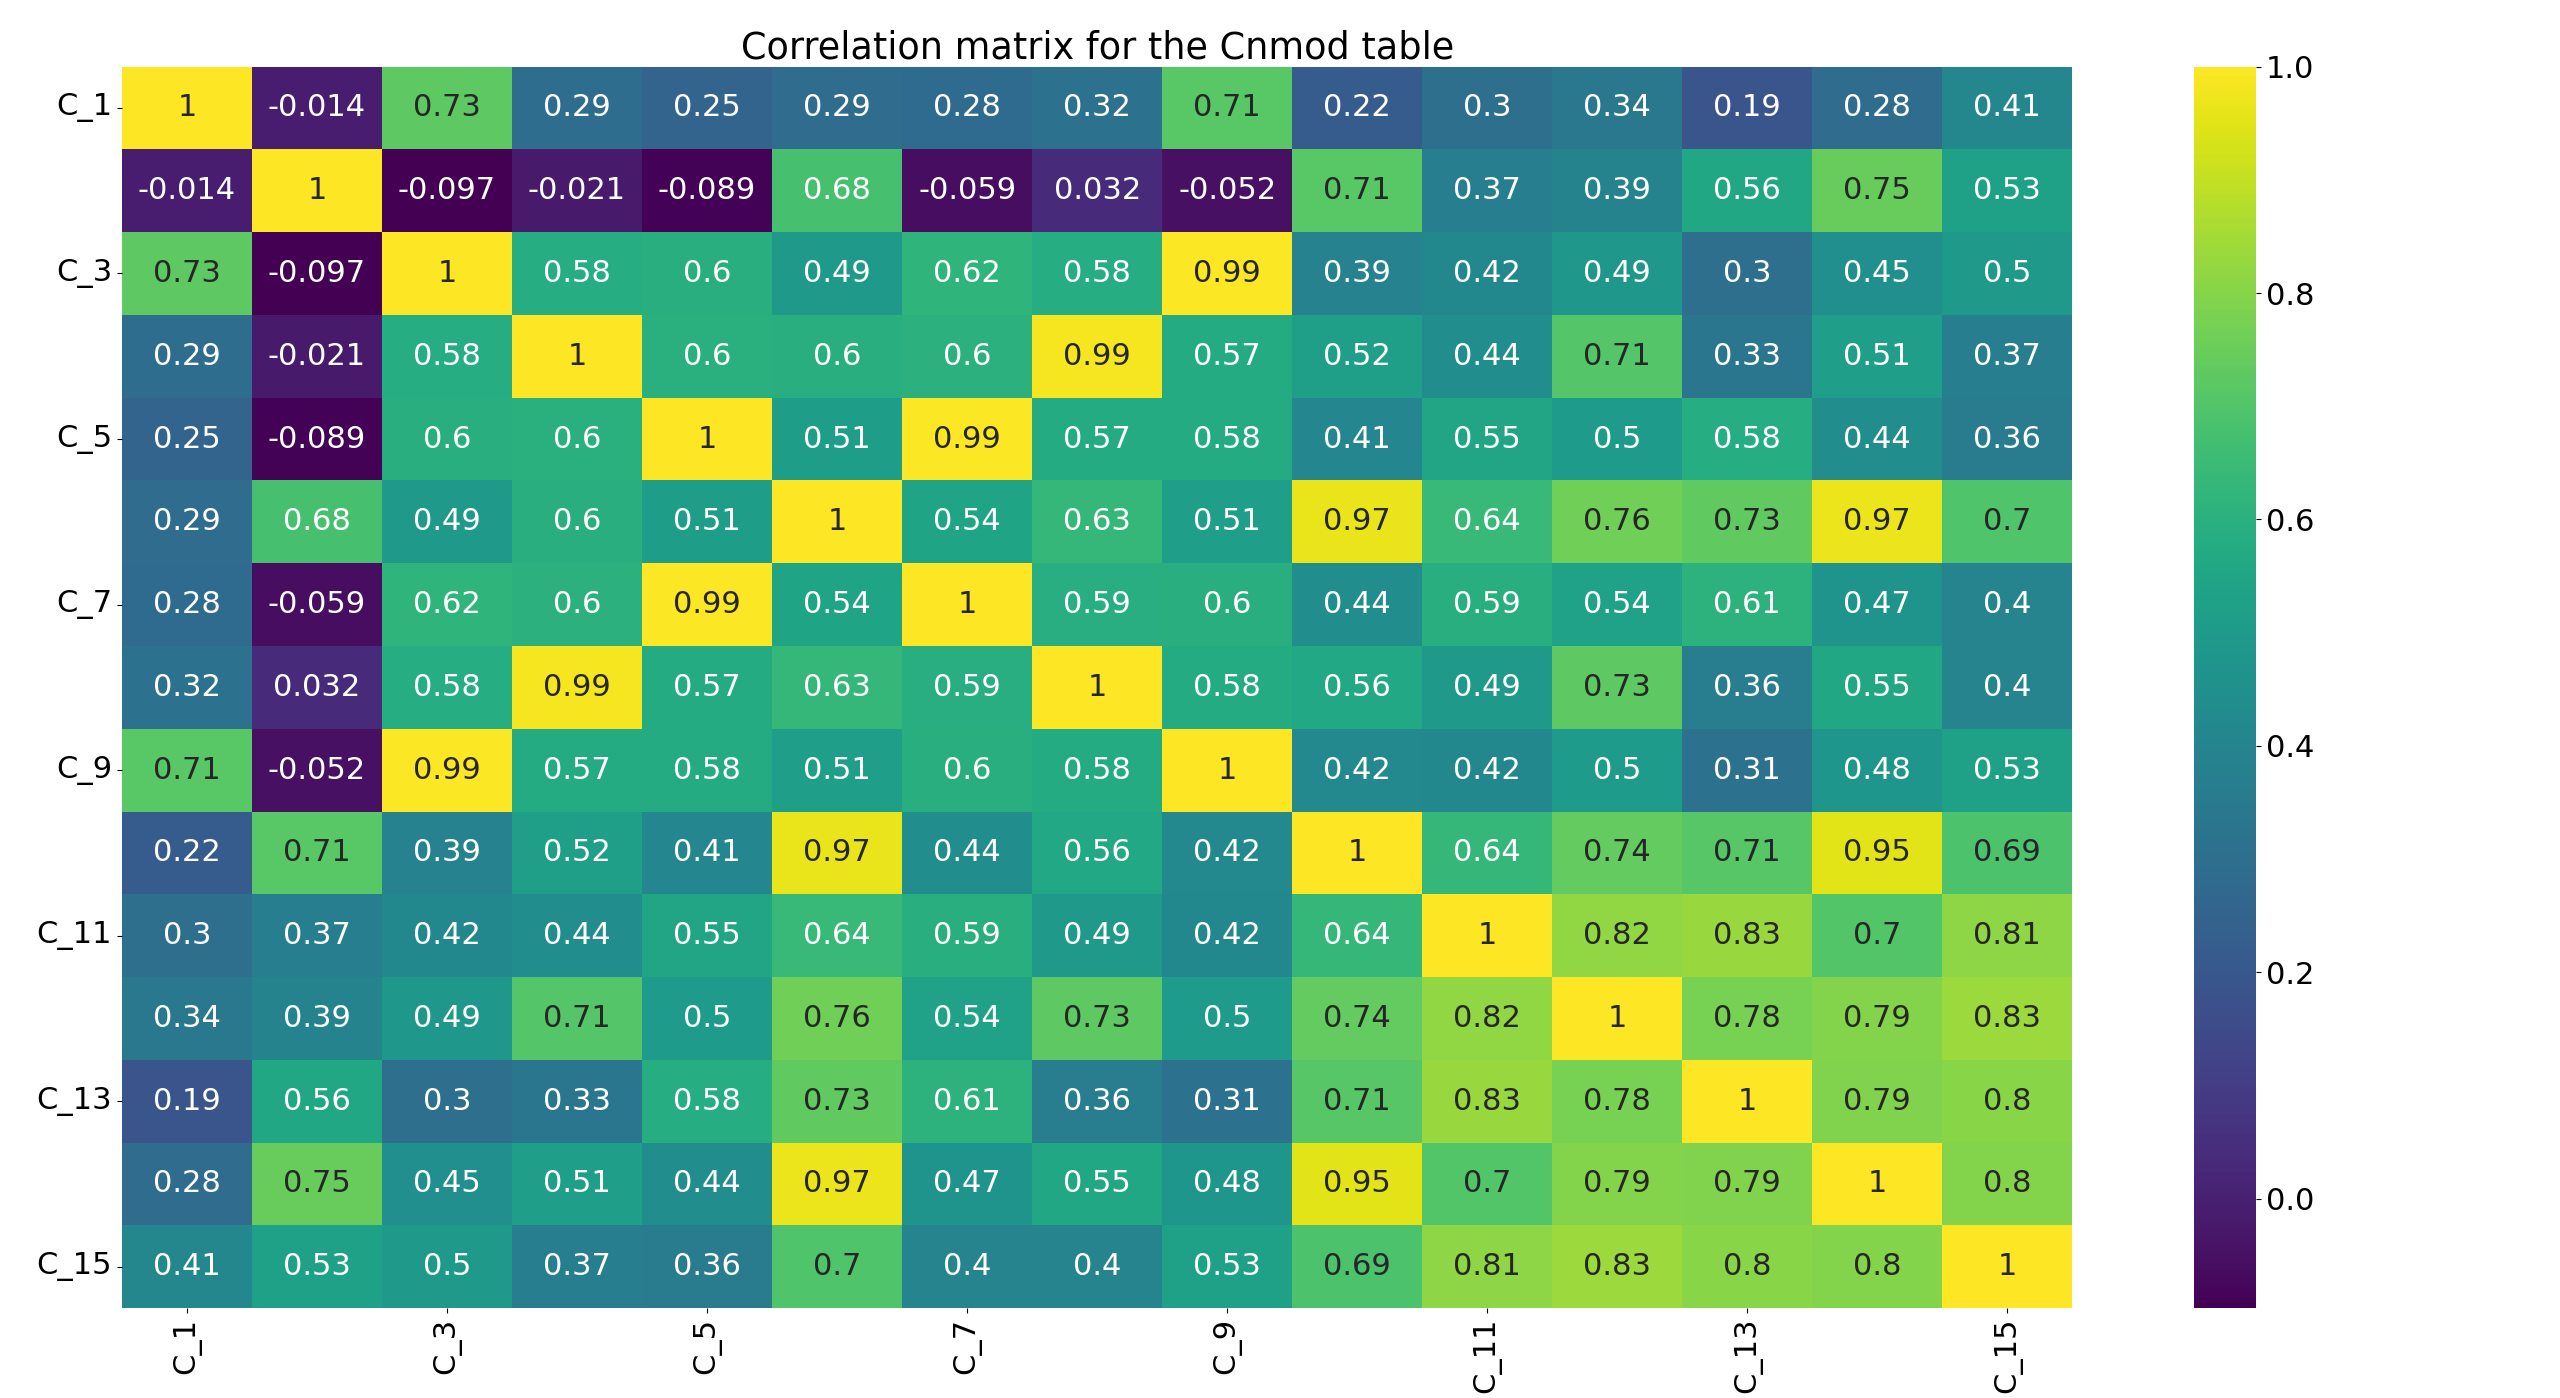
\includegraphics[width=\linewidth]{img/Cnmod_corr_matrix.png}
	\caption{The cross-correlation of the \cnmod\ harmonics} \label{fig:cnmod-corr}
\end{figure}

As we can see in \Cref{fig:cnmod-corr} the correlation matrix for \cnmod\ is very complicated:
\begin{itemize}
	\item Harmonic number $2$ is strongly correlated with any other harmonic until number $9$,
	\item Harmonics between $10$ and $15$ are strongly correlated among themselves,
	\item Harmonic number $4$ is strongly correlated with its multiples.
\end{itemize}
\begin{figure}[h!]
	\centering
	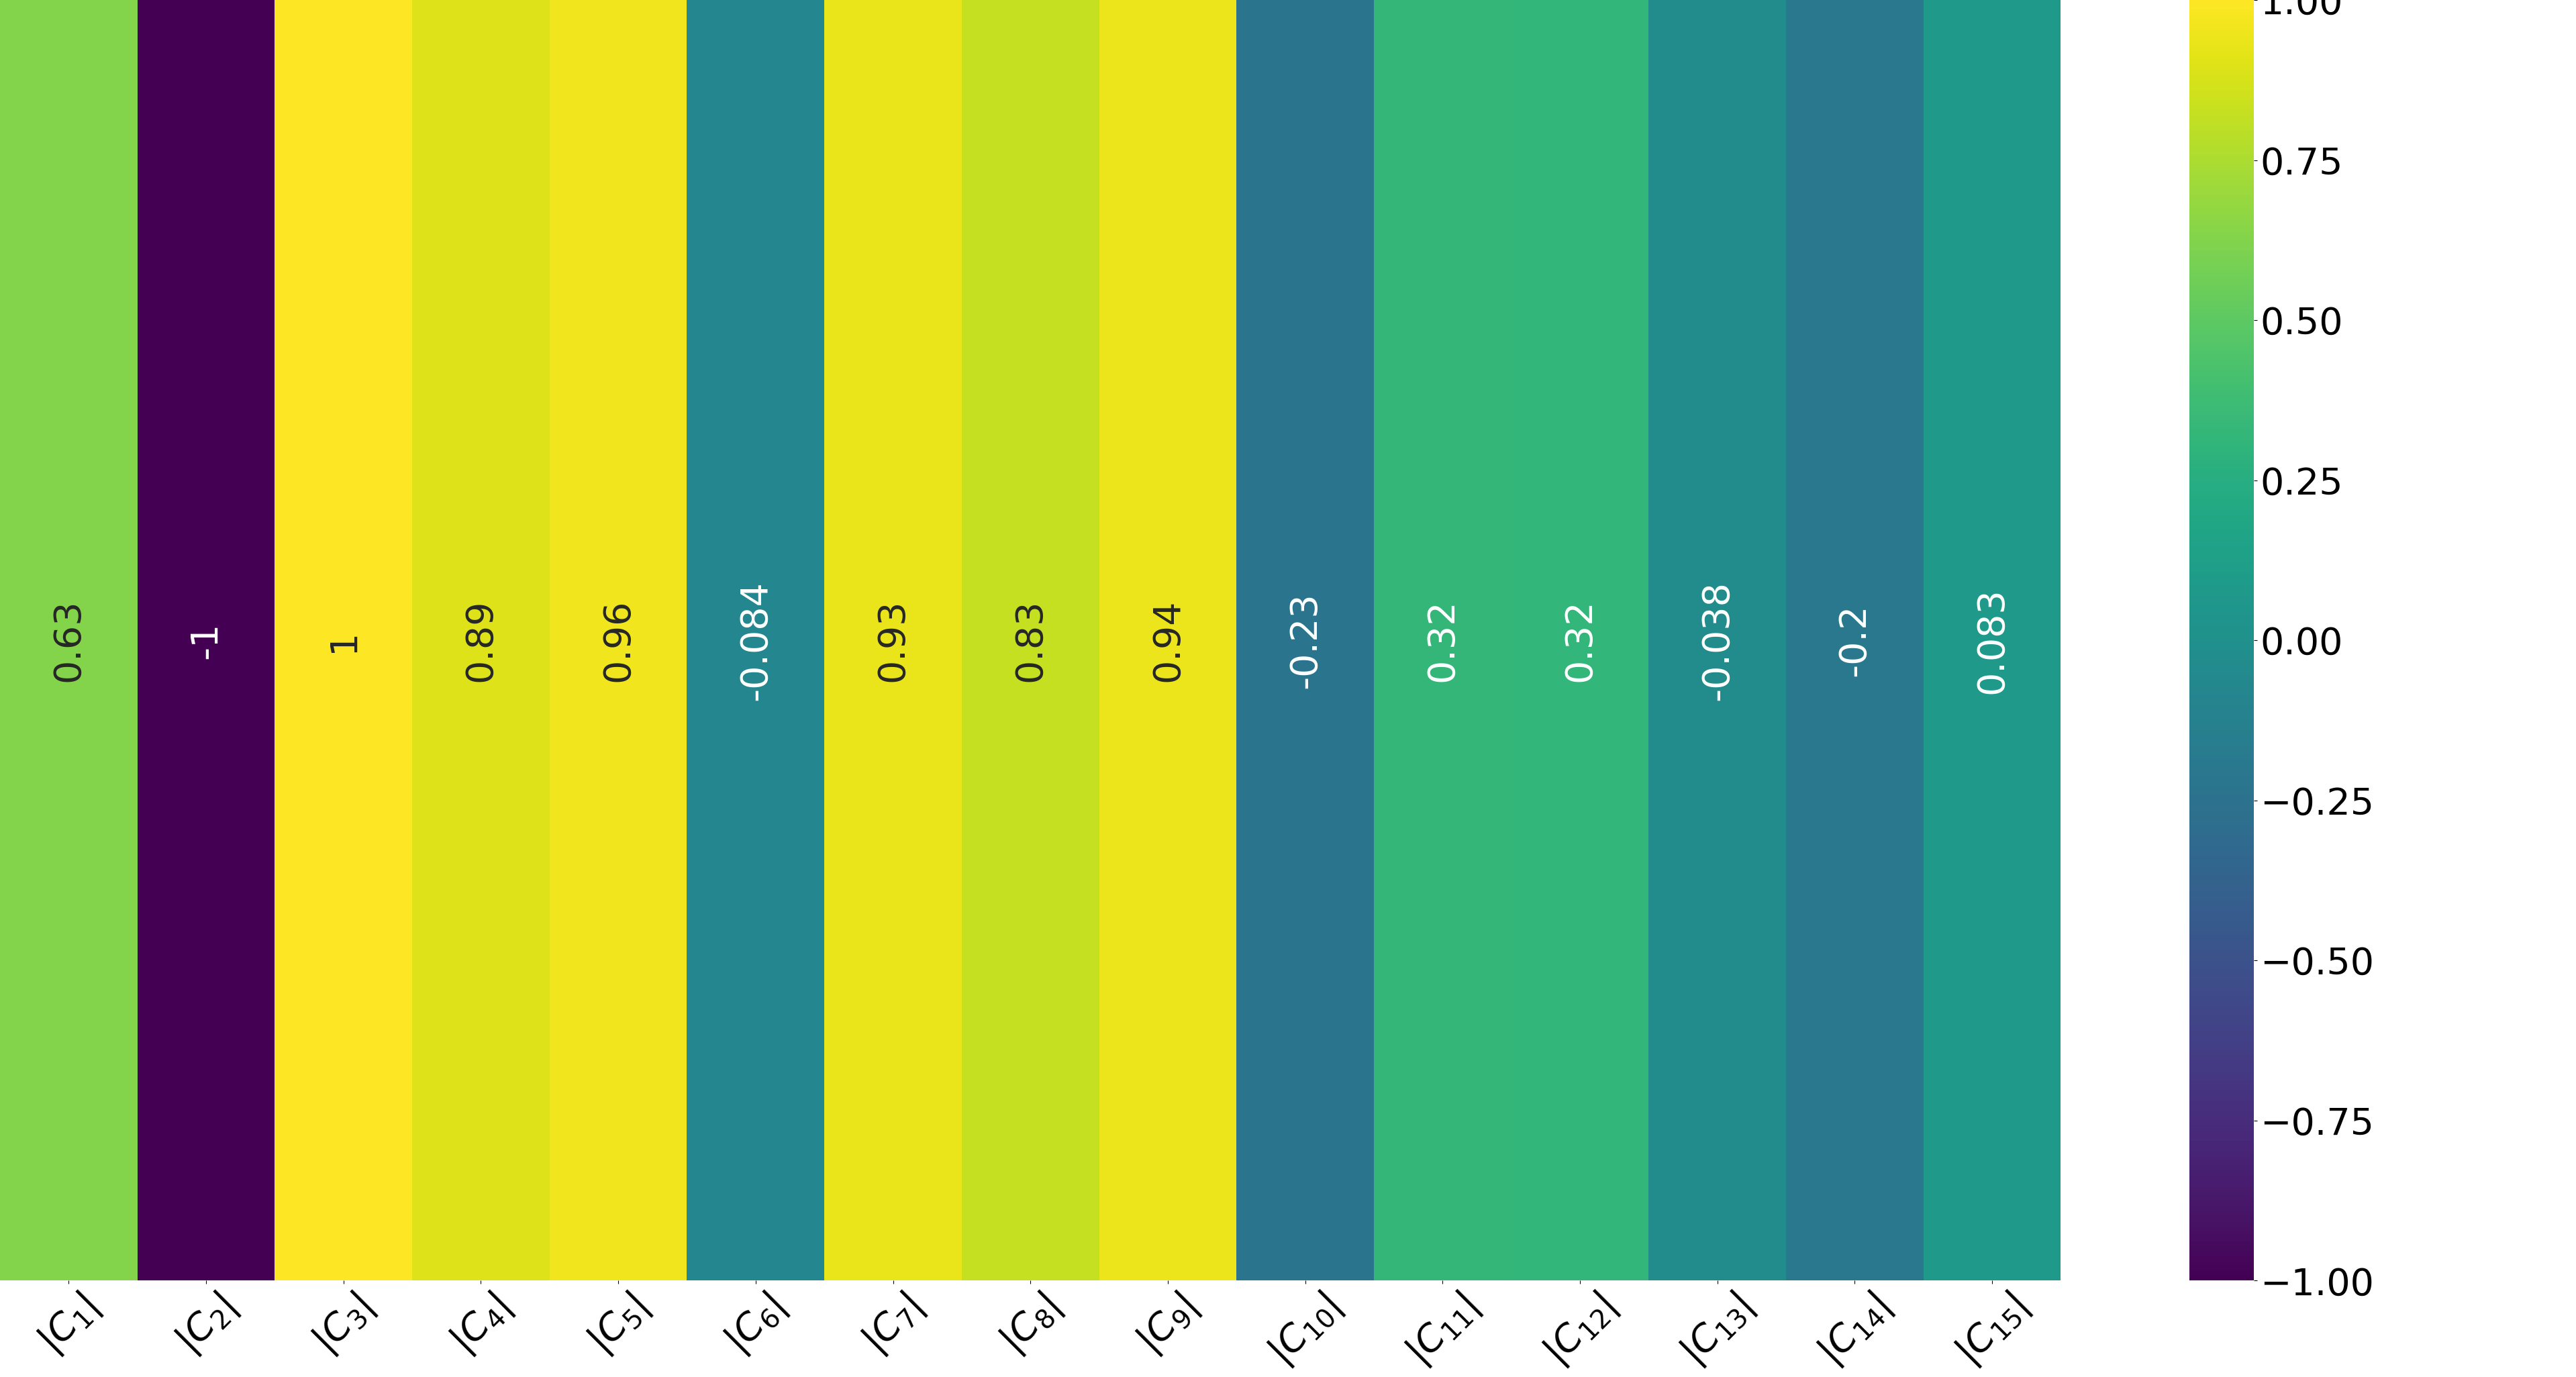
\includegraphics[width=\linewidth]{img/Cnmod_label_corr.png}
	\caption{Label correlation for the \cnmod table} \label{fig:cnmod-lcorr}
\end{figure}

Looking at both \Cref{fig:cnmod-corr} and \Cref{fig:cnmod-lcorr}, we can conclude that two different
approaches could be followed:
\begin{itemize}
	\item Using harmonic number $2$ alongside one or more high-order harmonics,
	\item Using harmonic number $3$ and some other low-order harmonics (potentially even the
	      first one) alongside one high-order harmonic (e.g., $14$).
\end{itemize}
Analyzing the boxplot suggested that using harmonic number $2$ was not promising, due to the extreme
concentration of the data.

Before considering the last table let us stop once more to consider the distribution of \cnmod\
after a round of \pca.
\begin{figure}[h!]
	\centering
	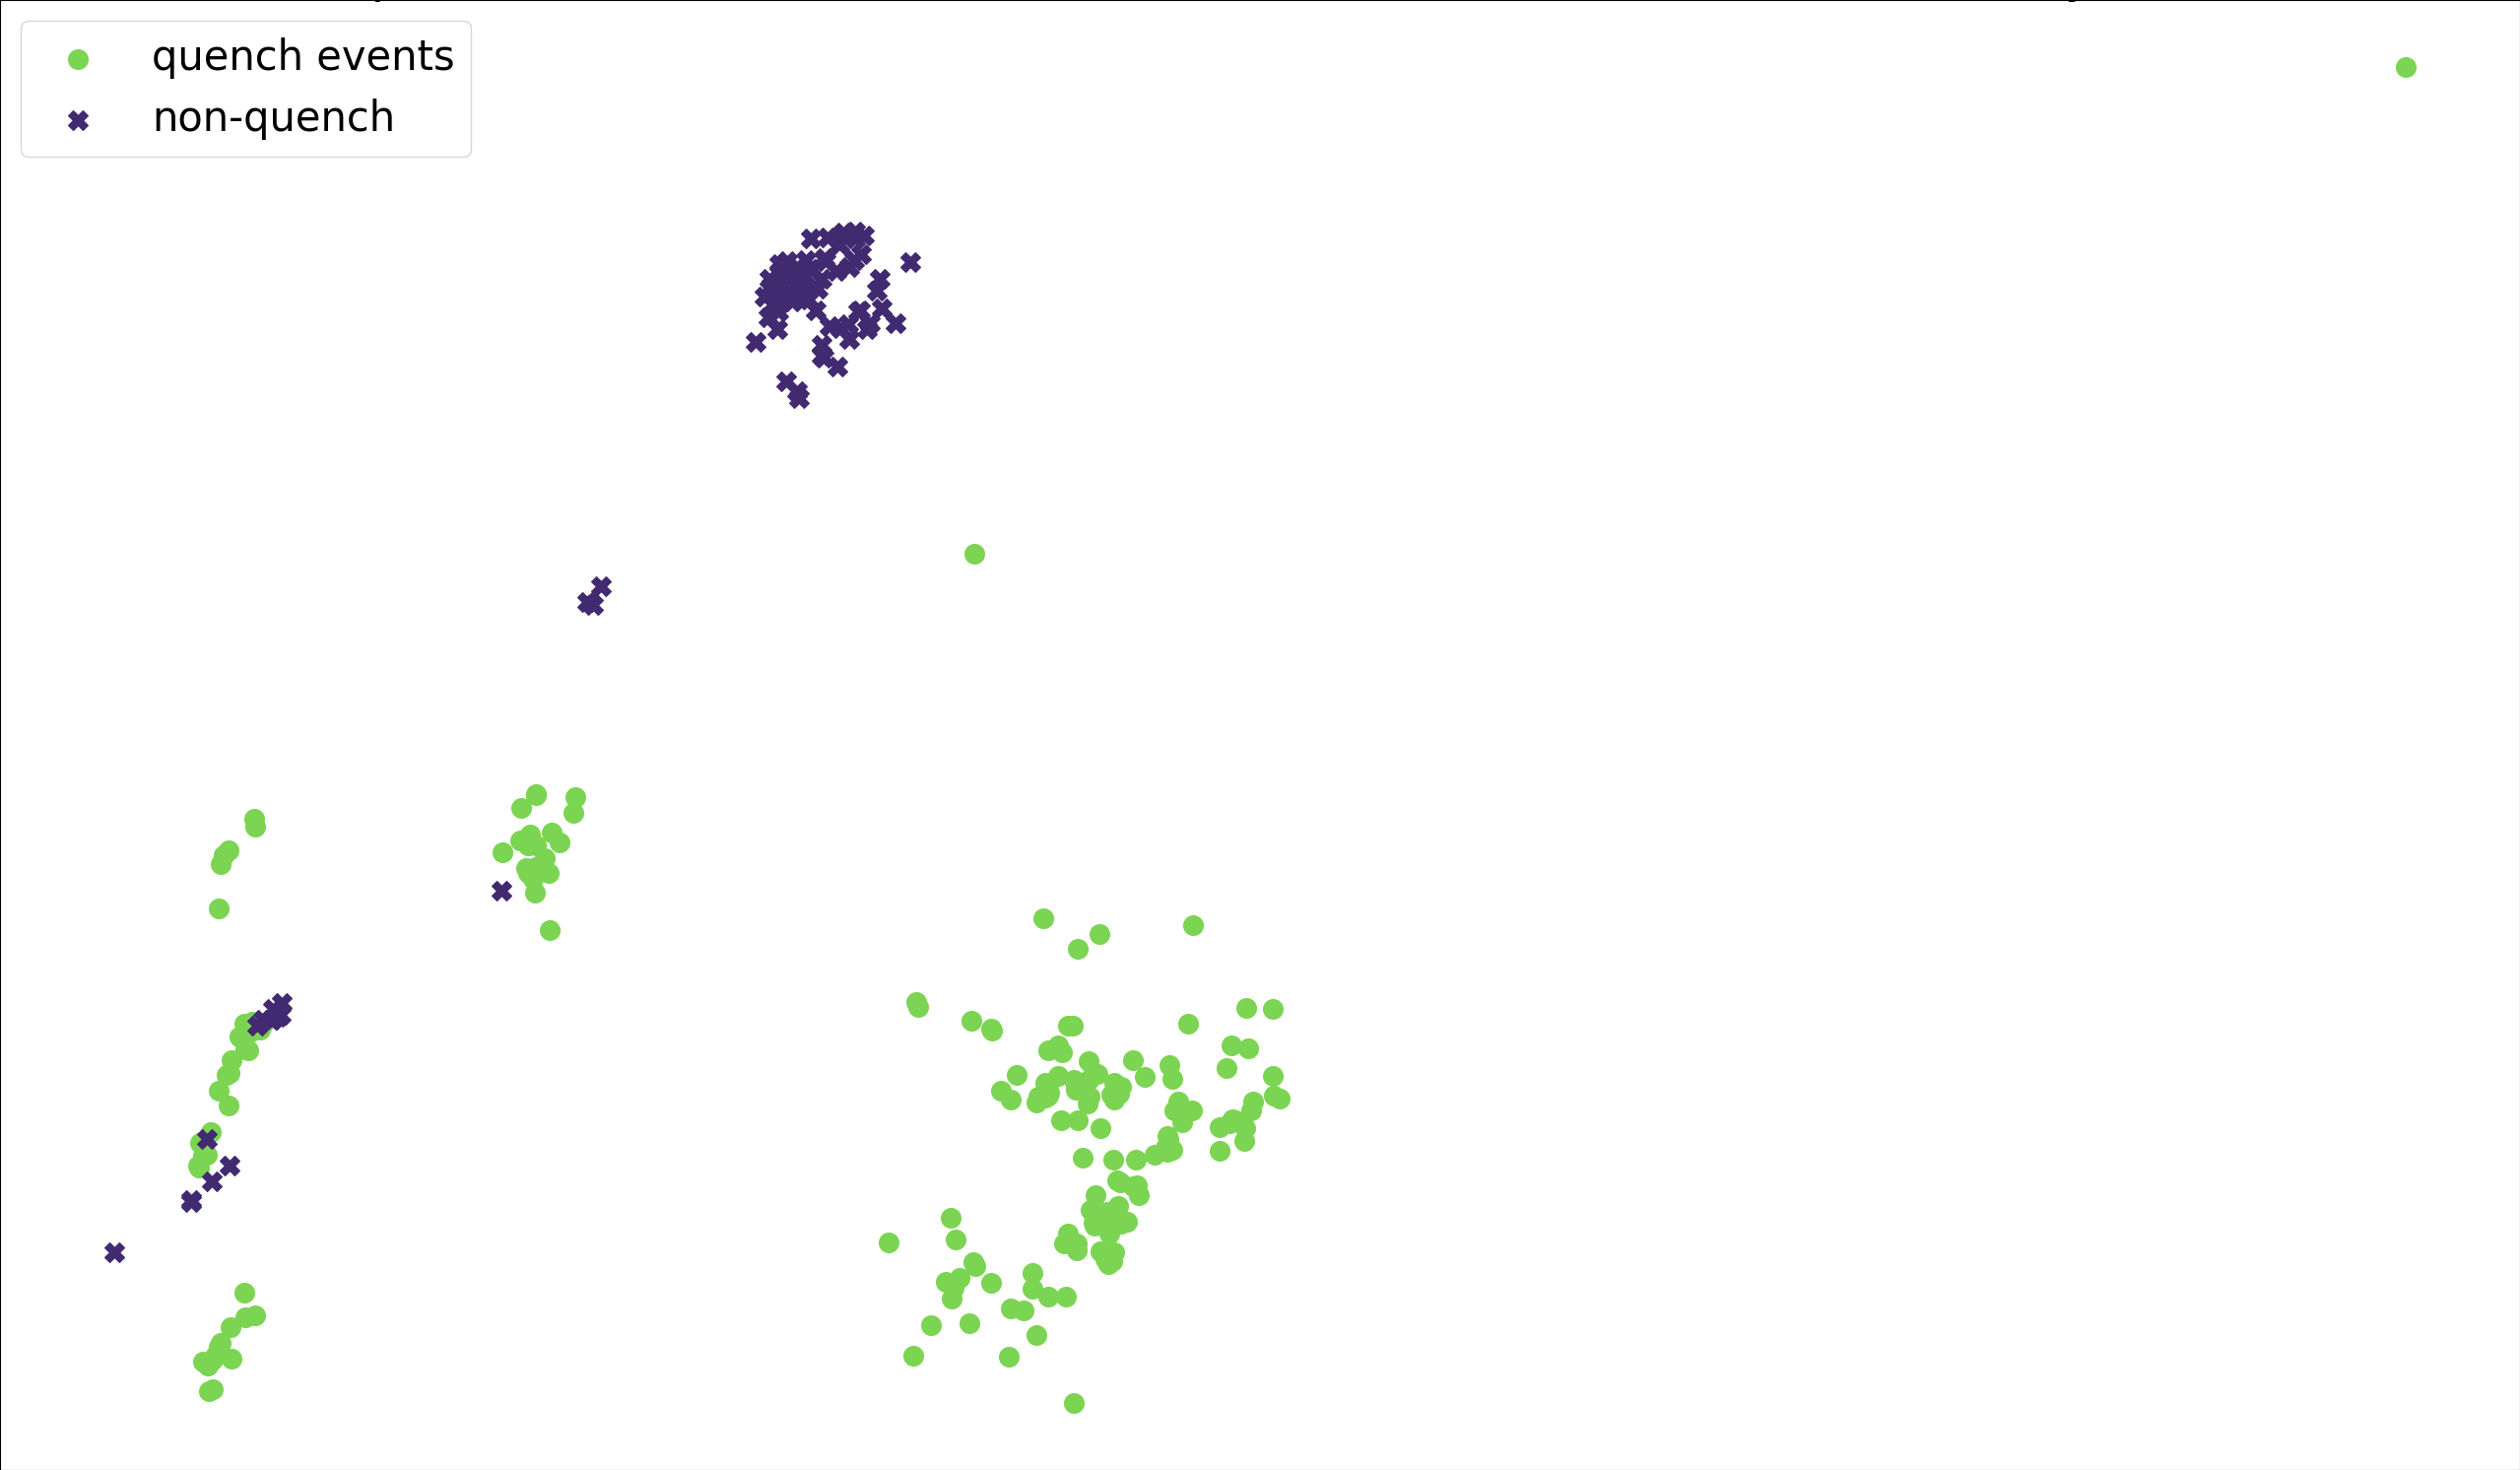
\includegraphics[width=\linewidth]{img/Cnmod_distribution.png}
	\caption{Data distribution for the \cnmod\ table after applying \pca\ dimensionality
		reduction} \label{fig:cnmod-dist}
\end{figure}
As we can see in \Cref{fig:cnmod-dist} the samples are characterized by a good enough distribution,
we could easily identify clusters with a high degree of purity, apart from the one in the leftmost
region of the image, which contains many points tagged as quench events and many points tagged as
non quenches. We can also identify a small outlier, which was removed when we considered the
clustering approach; overall \cnmod\ doesn't have a distribution quite as good as \an\ did, but
comparing it to \Cref{fig:bn-dist} or \Cref{fig:phi-dist}, has a much better topology.

\subsubsection{\phin\ table}
As we will see in further sections the \phin-based models consistently outperformed the ones based
on \bn. As we saw with \bn, also in the case of \phin, the data distribution after a round of \pca\,
shown in \Cref{fig:phi-dist}, is characterized by a series of high-impurity clusters where samples of the two
classes are mixed together.

\begin{figure}[h!]
	\centering
	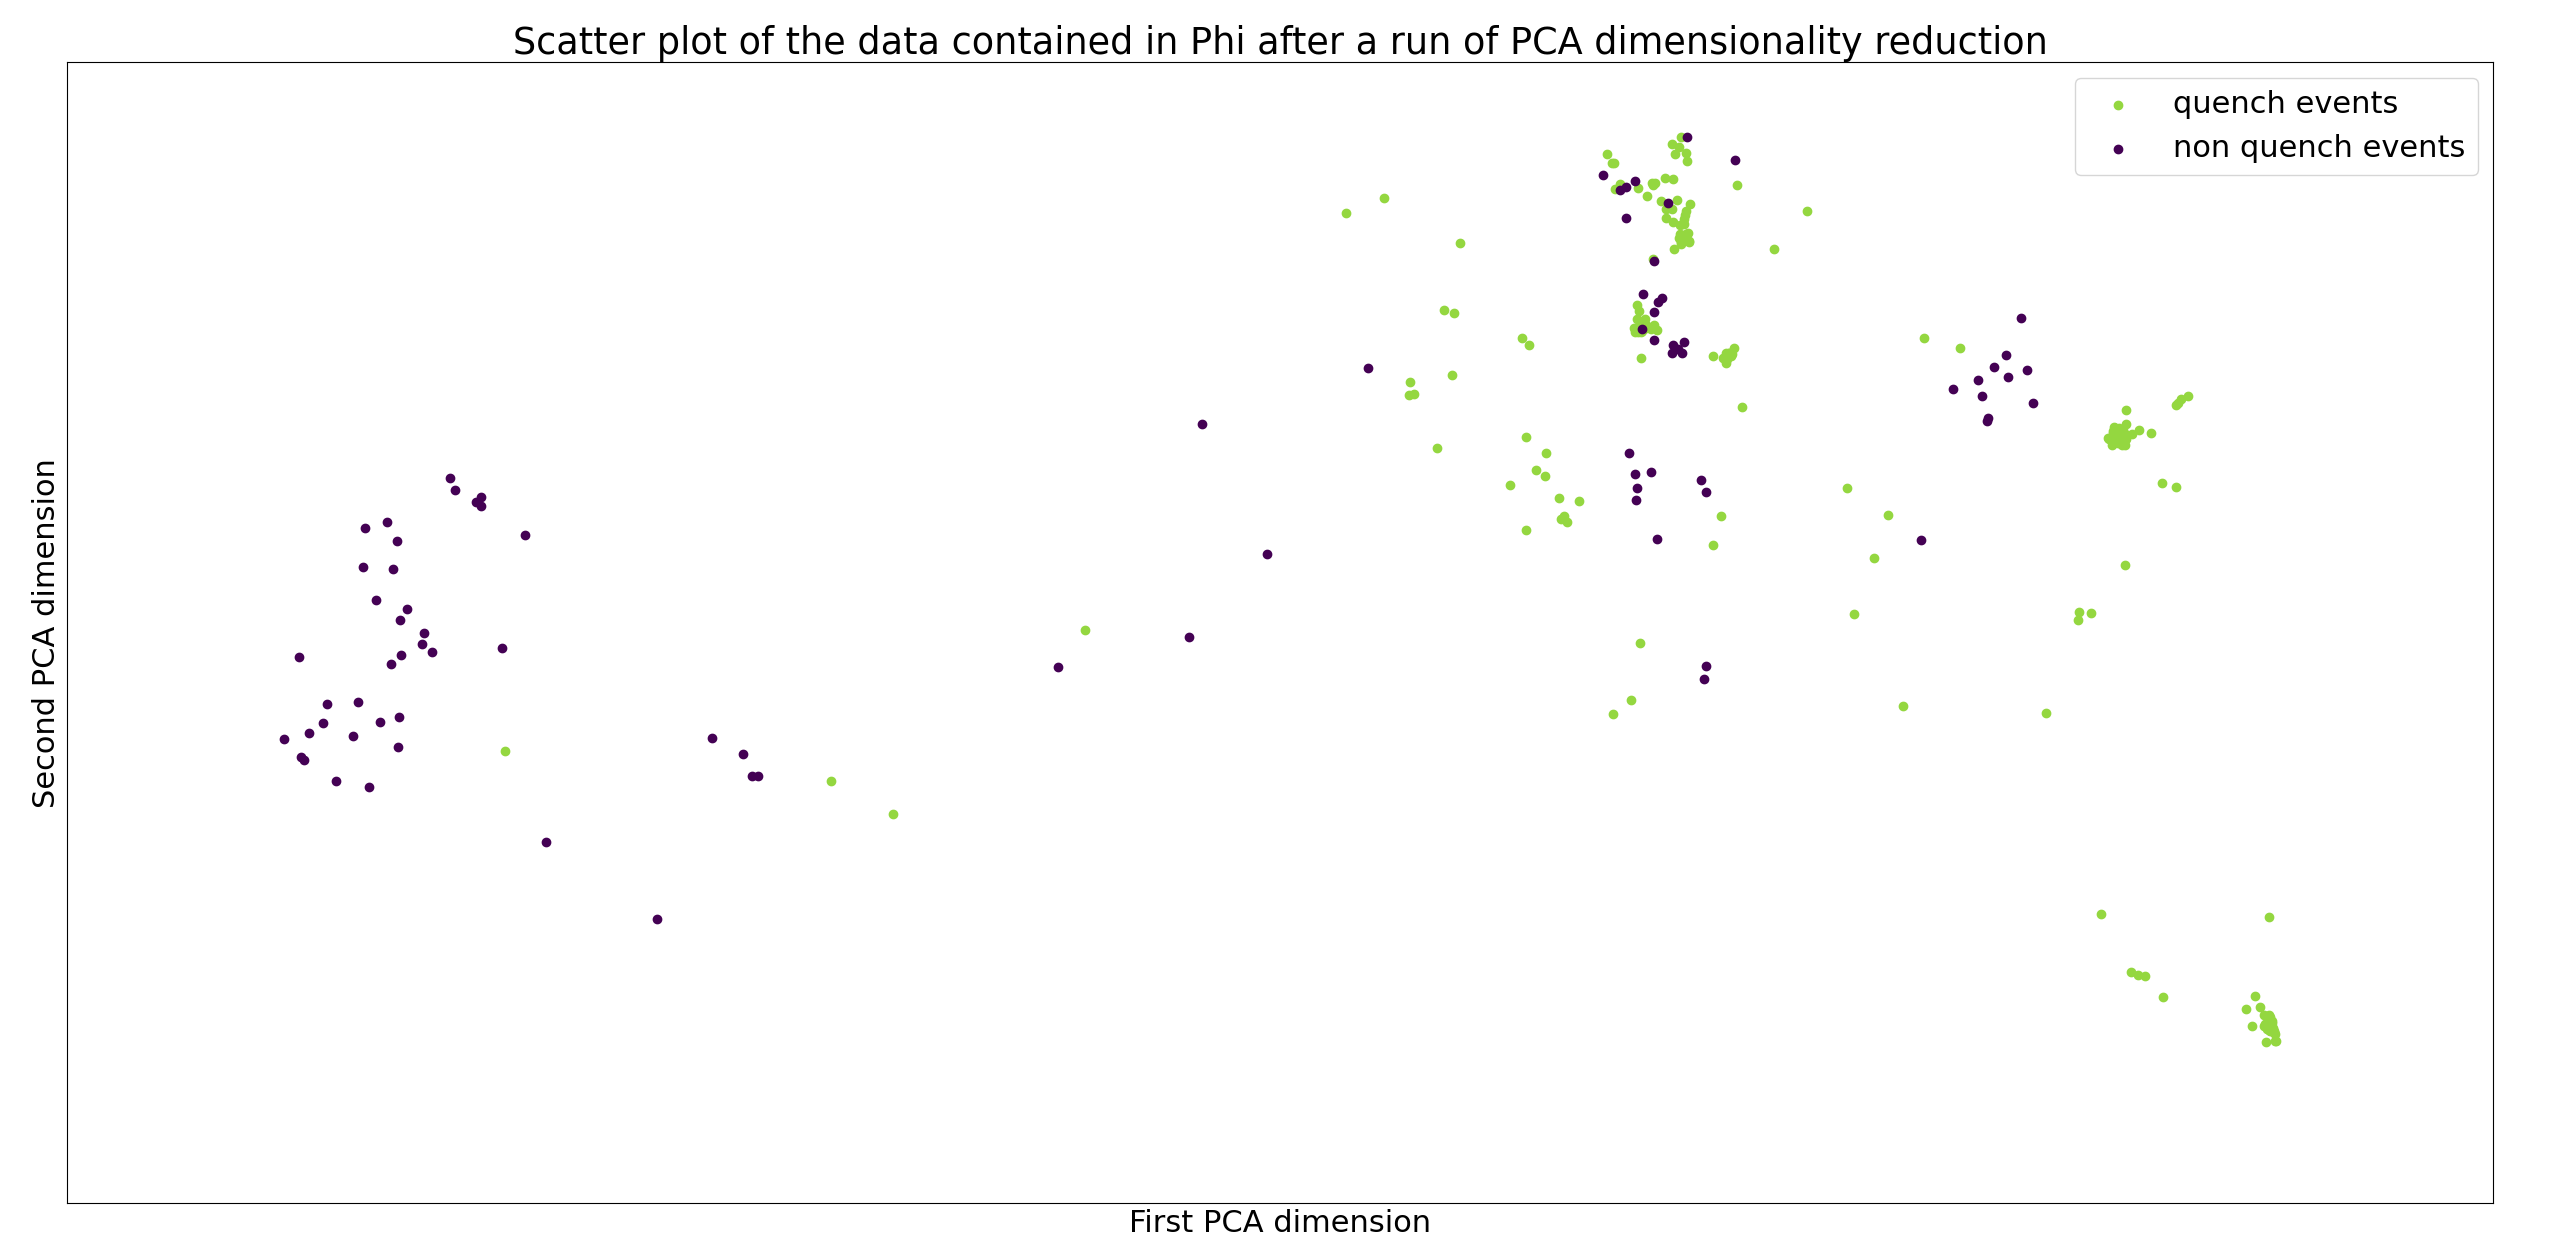
\includegraphics[width=\linewidth]{img/Phi_distribution.png}
	\caption{Data distribution for the \phin\ table after applying $\textsc{pca}$ dimensionality
		reduction} \label{fig:phi-dist}
\end{figure}

\medskip

As far as the correlation matrix is concerned we can see in \Cref{fig:phi-corr} that, contrarily to
the correlation matrix of other tables, the amount of harmonics that are strongly correlated with
each other is very low. No real structure can be seen in this table, as was the case of \an\ and \bn.
\begin{figure}[h!]
	\centering
	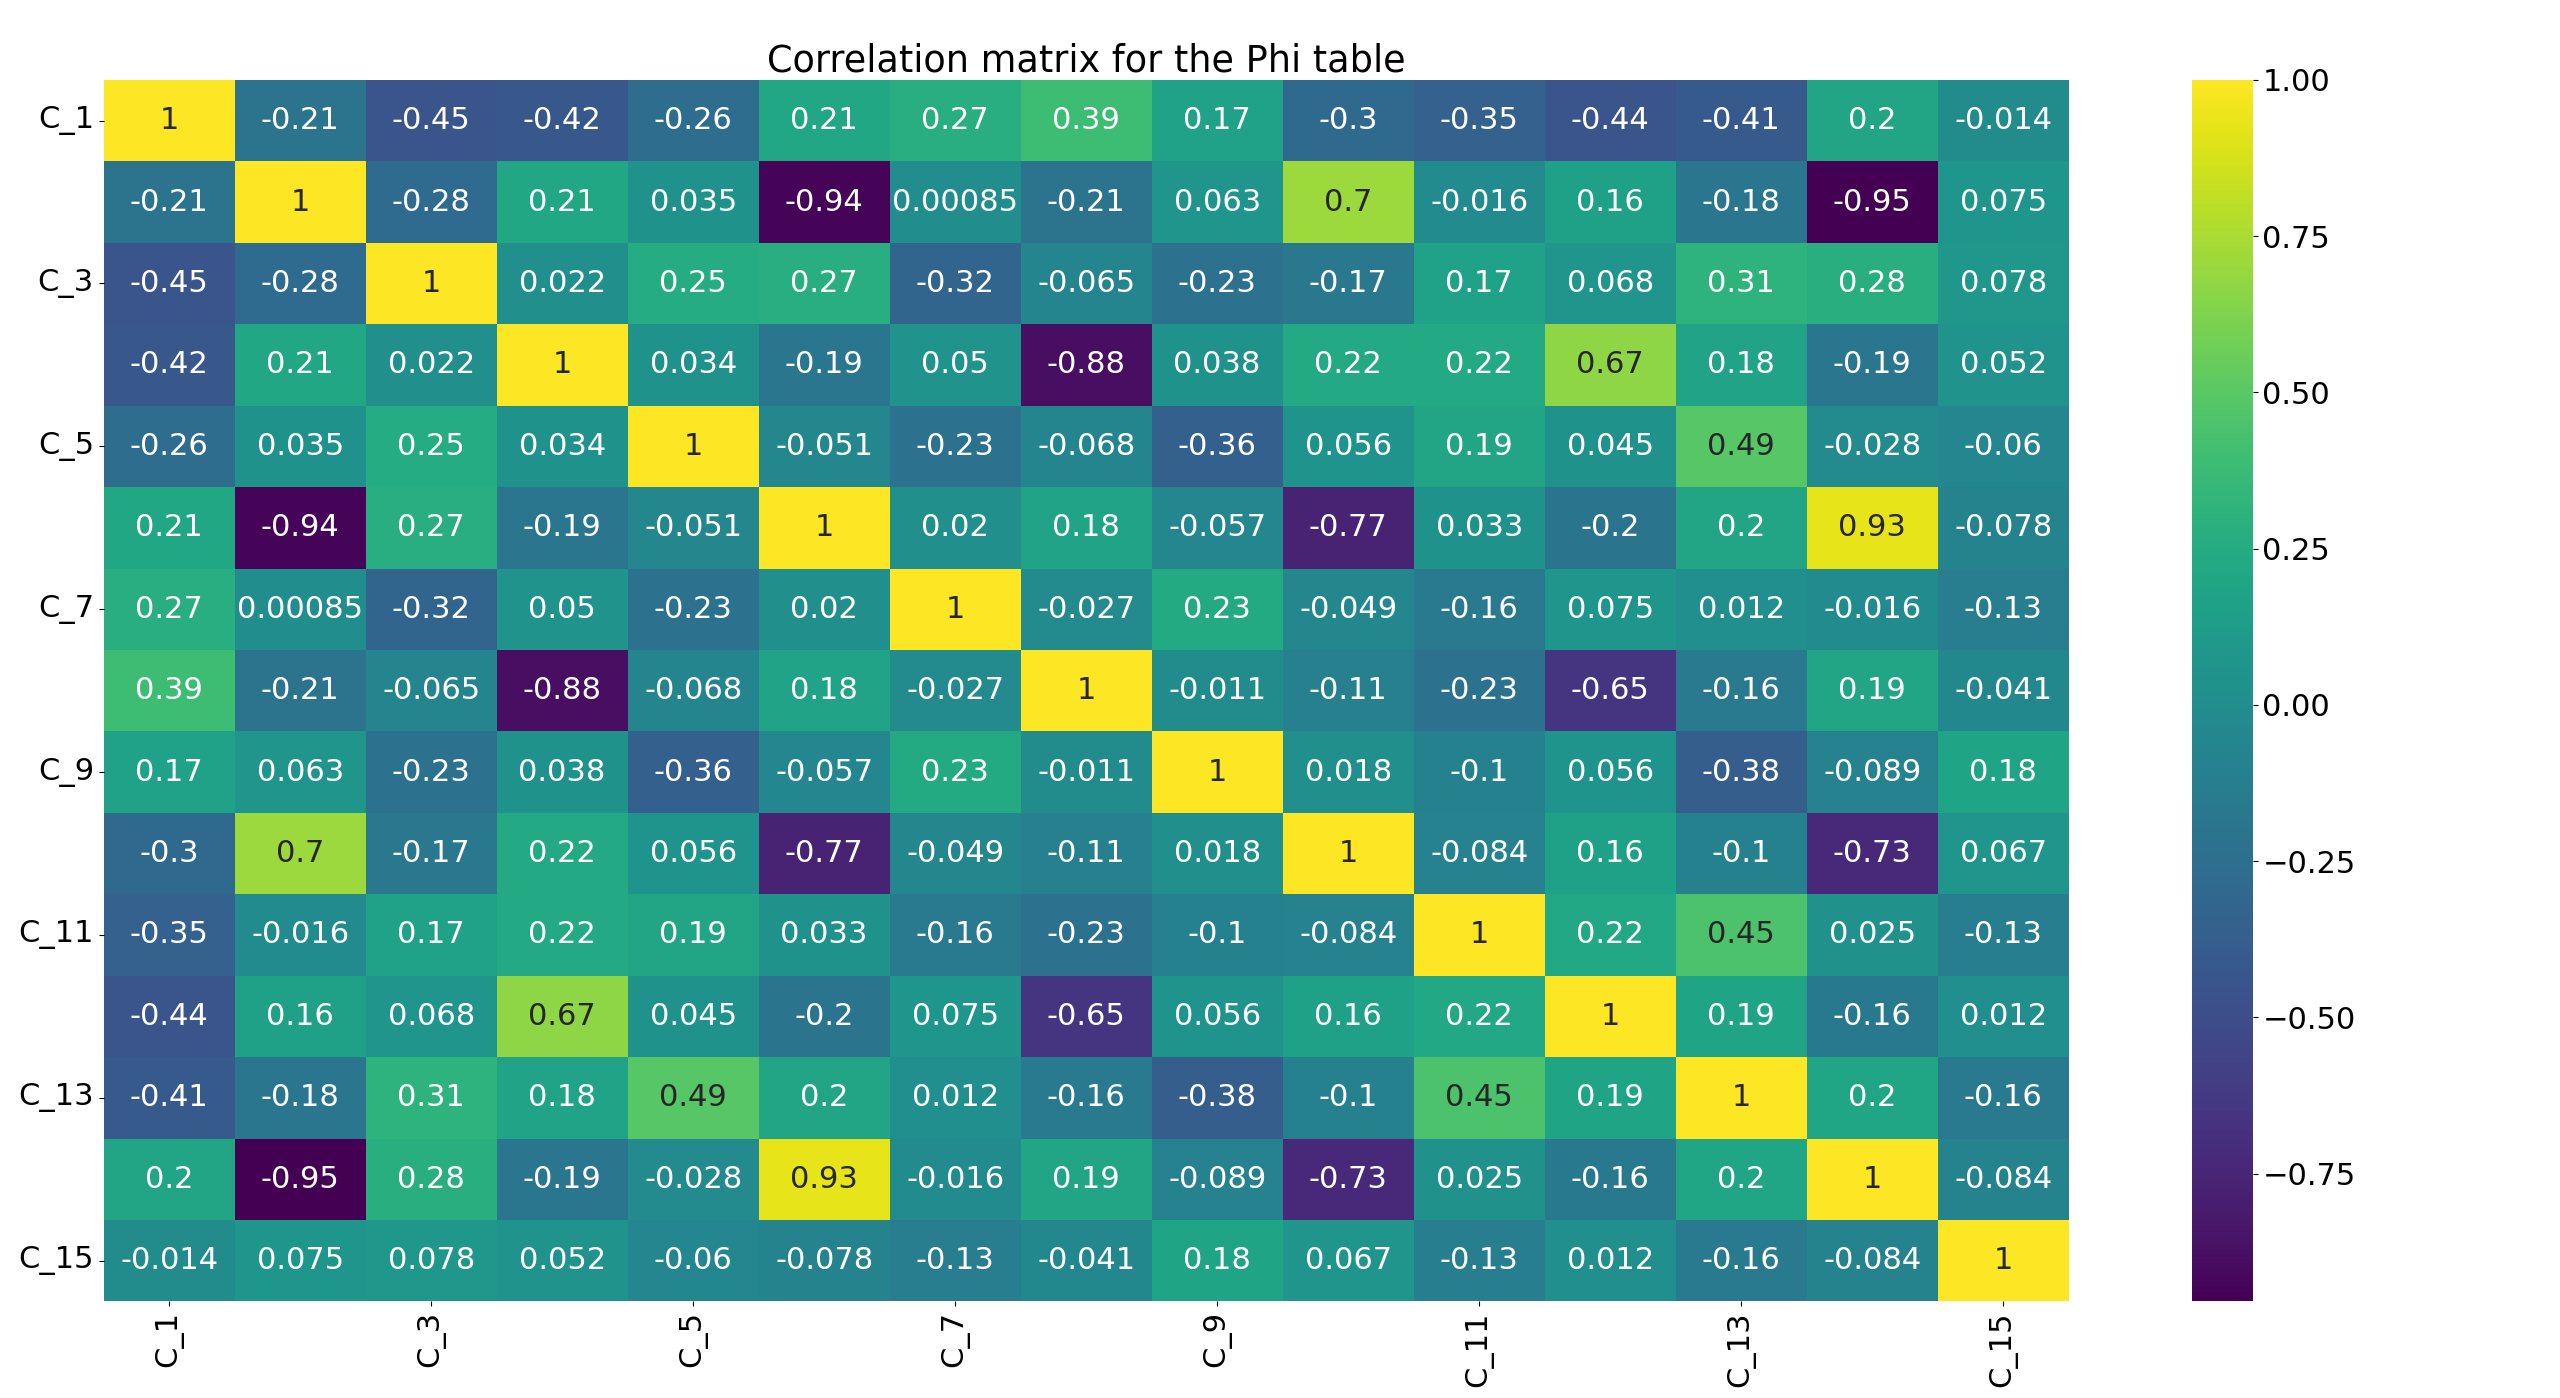
\includegraphics[width=\linewidth]{img/Phi_corr_matrix.png}
	\caption{The cross-correlation of the \phin\ harmonics} \label{fig:phi-corr}
\end{figure}
Whenever we choose to use \phin\ to build datasets we are left with much more freedom during the
feature extraction process, the only things that really stand to the eye are that:
\begin{inparaenum}[(i)]
	\item Harmonic number $2$ is strongly correlated with its odd multiples,
	\item harmonic number $4$ is strongly correlated with its multiples.
\end{inparaenum}

Lastly, we can analyze the correlation between the harmonics and the label. As we can see in \Cref{fig:phi-lcorr} most of the harmonics have a good correlation with the expected solution, especially harmonic number $2$ and its odd multiples, and harmonics number $1$ and $12$.
\begin{figure}[h!]
	\centering
	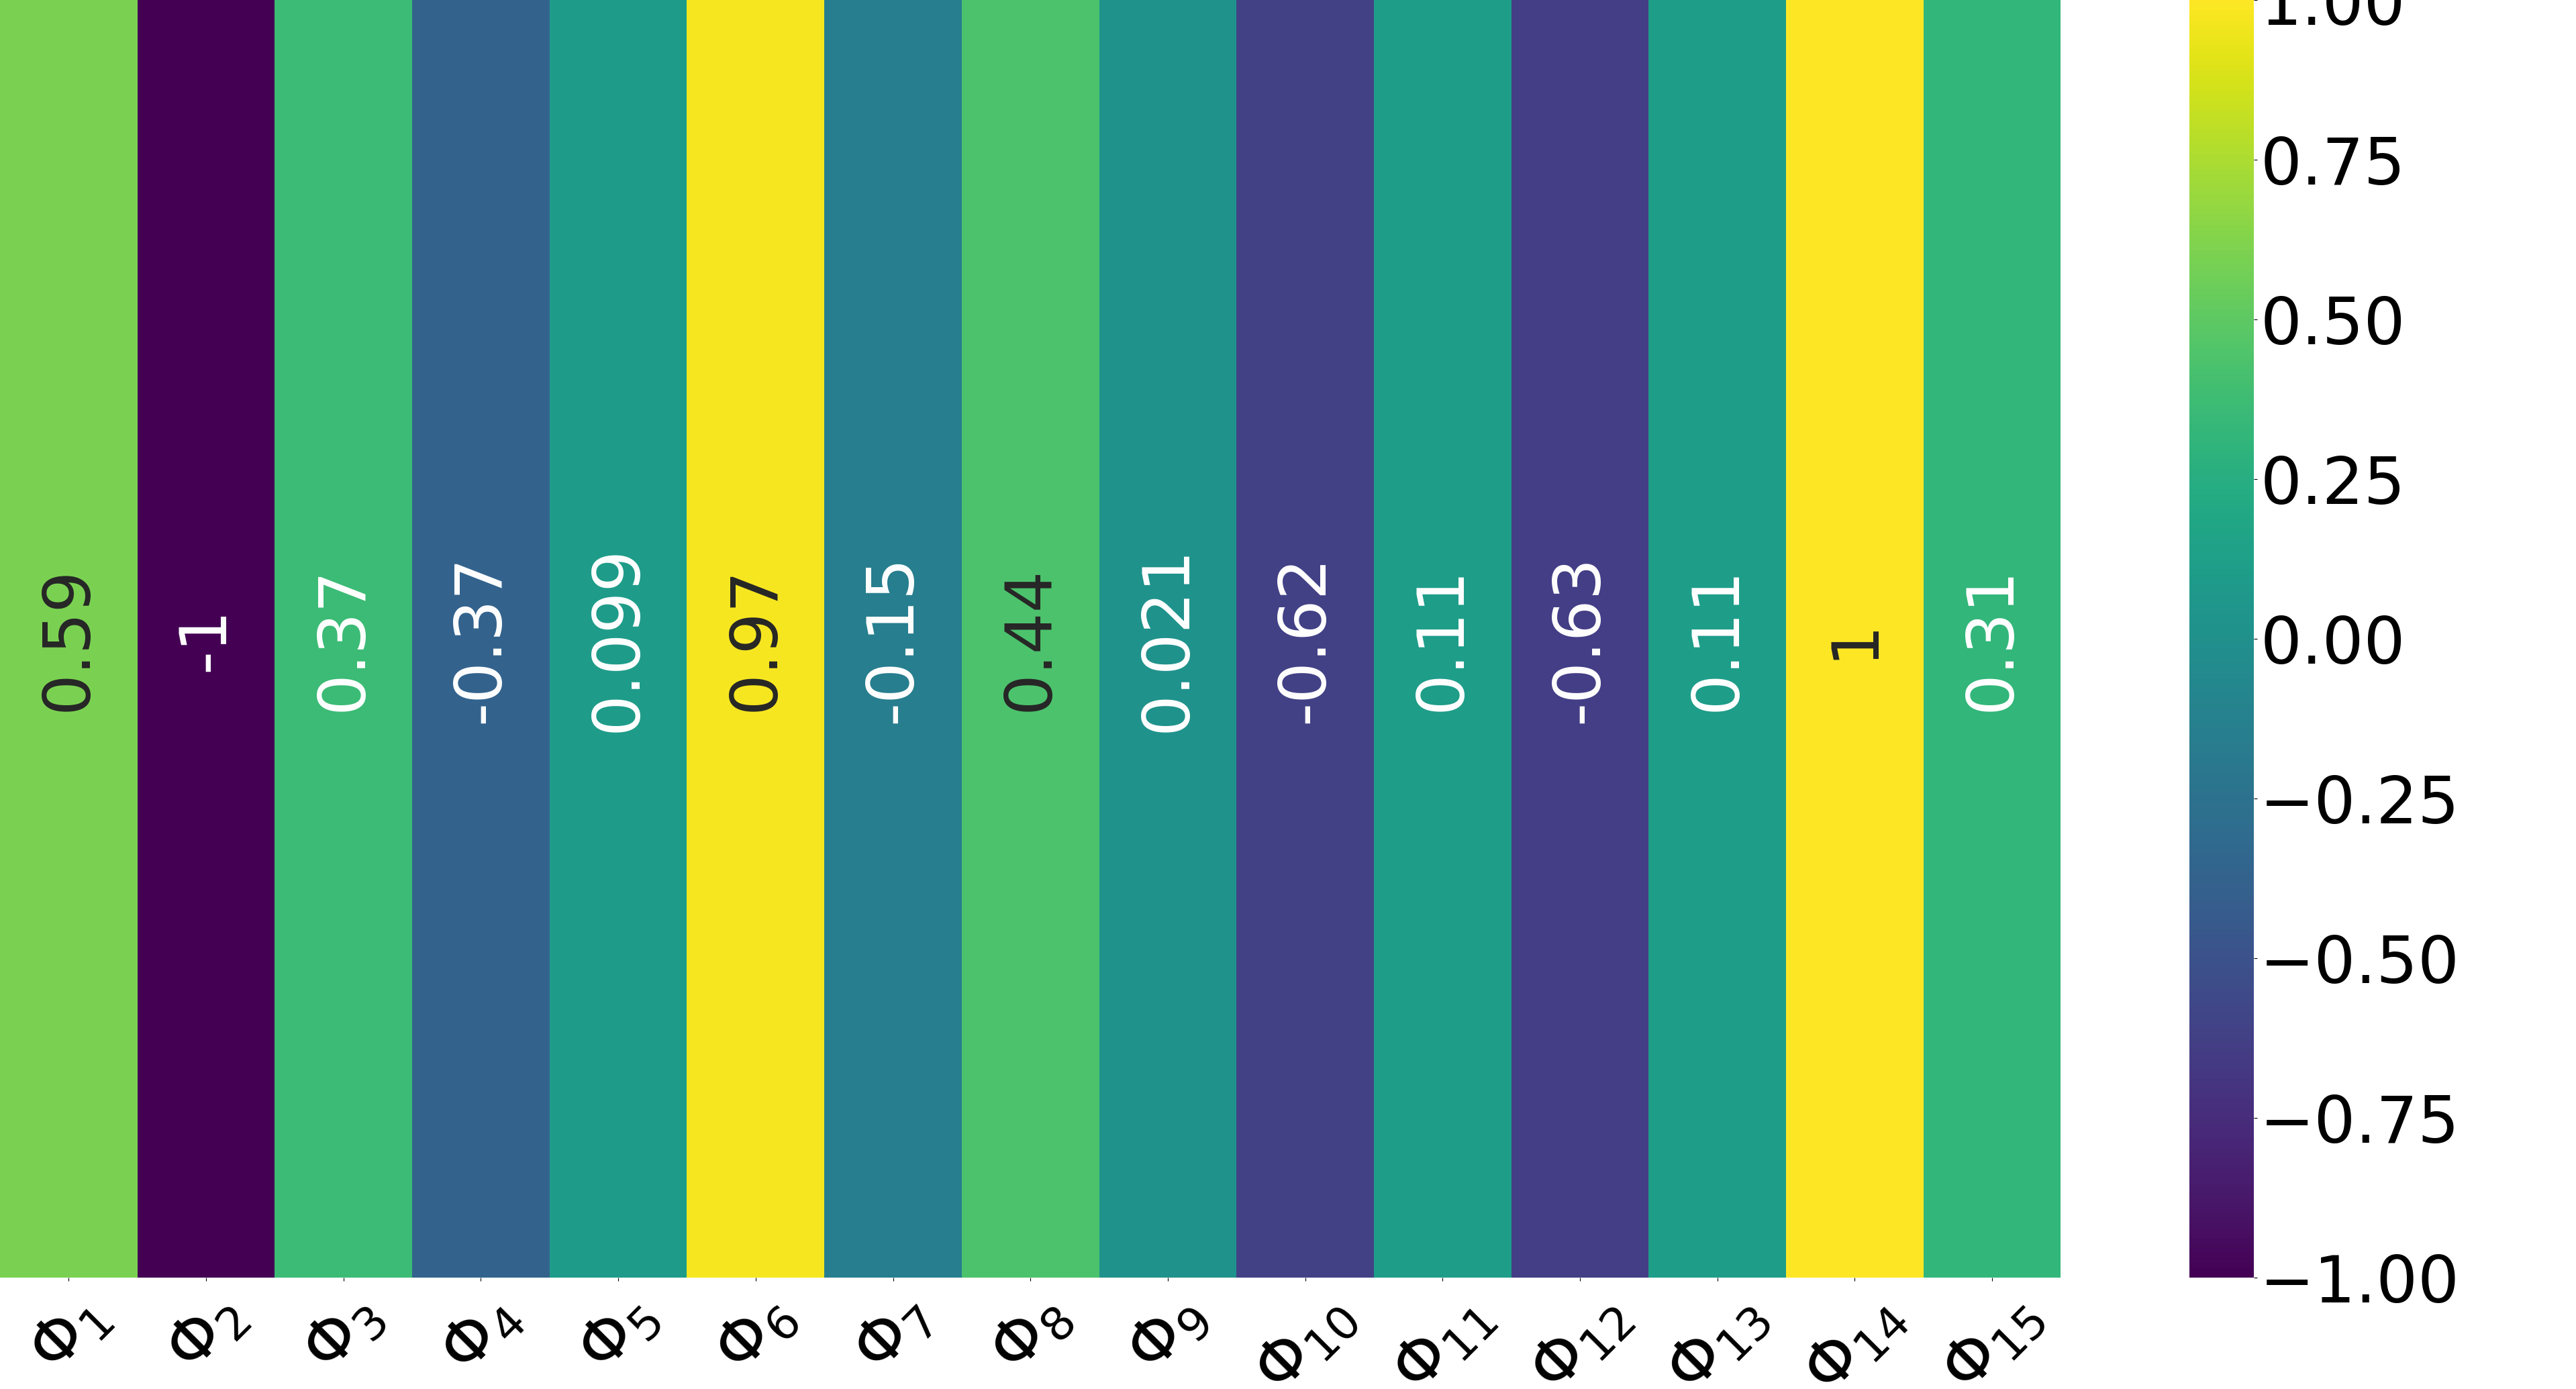
\includegraphics[width=\linewidth]{img/Phi_label_corr.png}
	\caption{Label correlation for the \phin\ table} \label{fig:phi-lcorr}
\end{figure}

This closes the brief exposition about the preprocessing steps for the various labels, now we will
tackle the model selection procedure indicating which were the best models overall and which model
we chose to solve \qrp.

\section{Results}
Every model shown in this section has been tested using the pipeline that we introduced in
\Cref{chp:problem}. In this chapter we will proceed as we did in \Cref{chp:ml} for the theoretical
introduction of the models, therefore:
\begin{itemize}
	\item The first subsection delineates the performance of decision trees,
	\item The second subsection delineates the performance of random forests,
	\item The third subsection delineates the performance of our benchmarking model, the \svm,
	\item The last subsection will introduce the tree aggregator model
\end{itemize}
At the end of the chapter we will talk about the best performing model and we will give the final
results for \qrp.

\subsection{Decision trees}
As we already alluded to in previous sections we wanted to find a highly explainable model with good
performance that could be used to solve \qrp, that is exactly why the development process started
with \dts.

With our experiments we tried different approaches and different datasets, after a careful analysis
and many experiments we found that the best \dts were all based on \an, the confusion matrix for
the best model, trained on harmonics $2$ and $12$, is shown in \Cref{fig:dt-an-2-12-cm}, as we can
see, the total number of errors made by the model is of only $4$ total, $3$ false negatives and $1$
false positive.
\begin{figure}[h!]
	\centering
	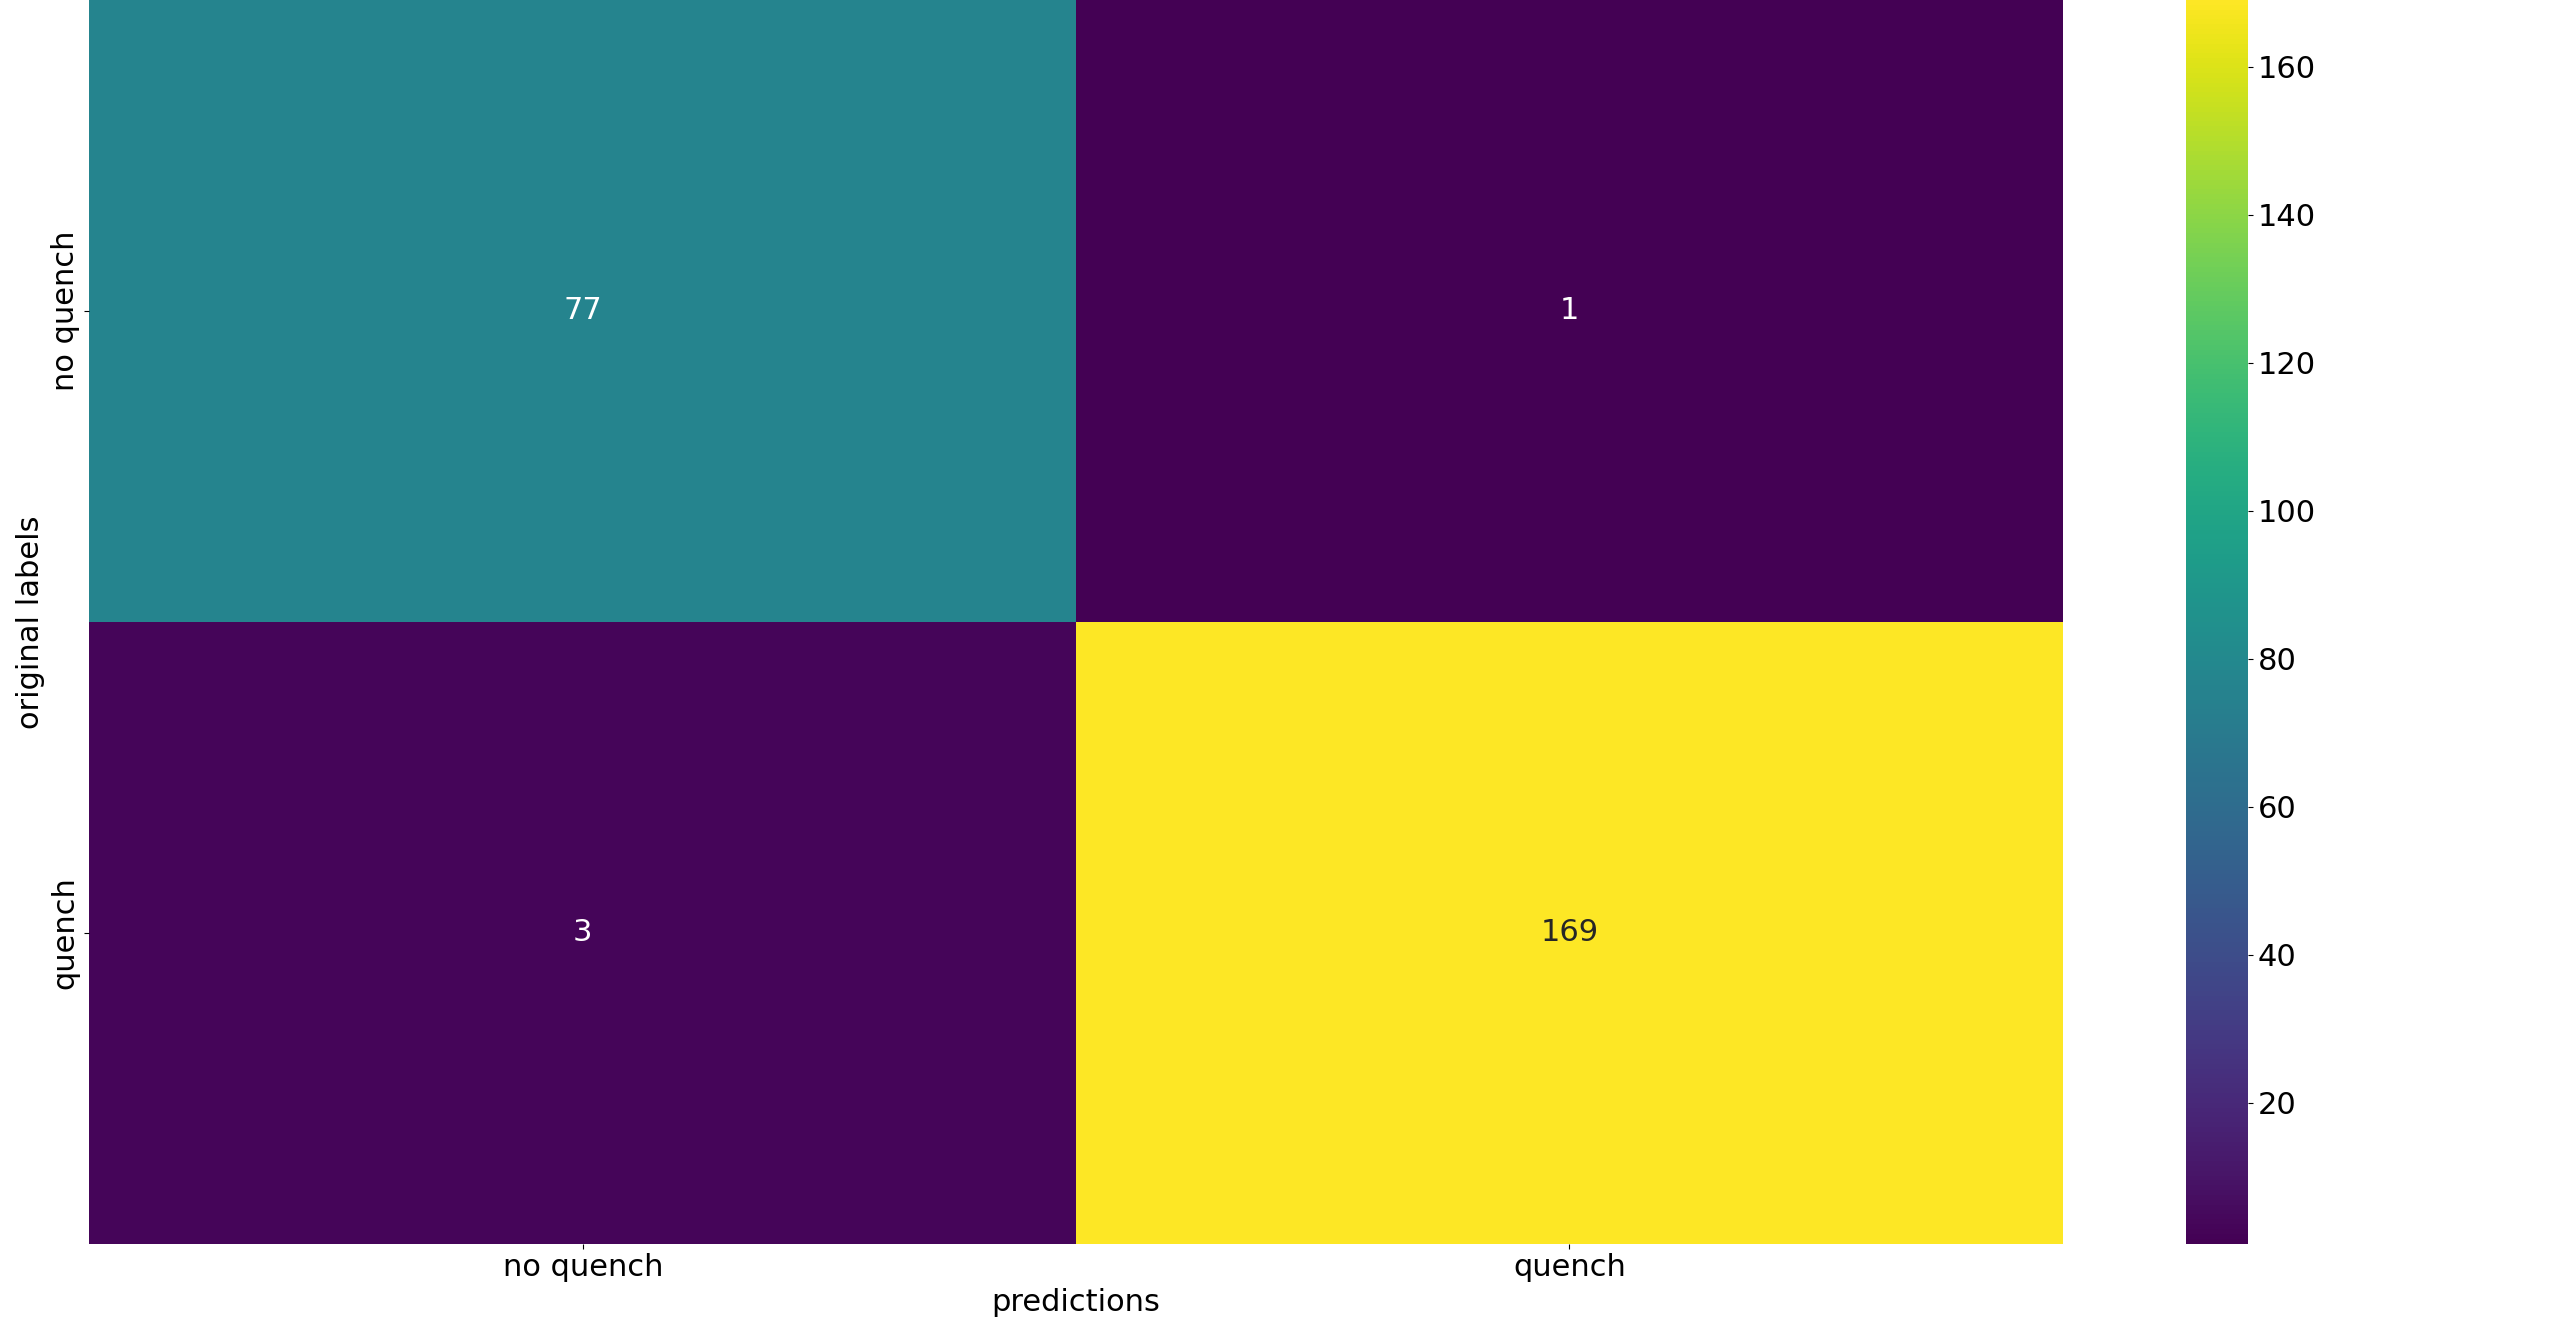
\includegraphics[width=\linewidth]{img/An_2_12_cm_dt.png}
	\caption{The performance for the \an model built on harmonics $2, 12, 15$}
	\label{fig:dt-an-2-12-cm}
\end{figure}
The average performance of the model over the outer \cv\ folds is reported in \Cref{tbl:an-2-12-perf},
as we can see, the numbers are already very solid, showing high average fold performance and low
standard deviation.
\begin{table}[t]
	\caption{Average and standard deviation of the performance for the best \dt\ over the outer \cv\
		fold.}\label{tbl:an-2-12-perf}

	\bigskip
	\setlength{\tabcolsep}{6pt}
	\centering
	\begin{tabular}{ccccccc}
		\toprule
		\textbf{}    & \textbf{Acc} & \textbf{Prc} & \textbf{Rec} & \textbf{Irec} & \textbf{F1} & \textbf{RAUC} \\
		\midrule
		Mean         & 0.984        & 0.994        & 0.983        & 0.988         & 0.988
		             & 0.989                                                                                    \\
		\textsc{std} & 0.008        & 0.011        & 0.014        & 0.025         & 0.006
		             & 0.012                                                                                    \\
		\bottomrule
	\end{tabular}
\end{table}
These results are telling us that the model is able to perform on a high level in all of the testing
metrics that we have chosen, moreover it's telling us that the delta, for every metric, between the
best and the worst fold is very quite small, meaning that the model performed quite similar in all
testing folds.

If we look at \Cref{fig:dt-an-2-12-pt}, we can see that the structure of the tree is also
extremely simple, contained in depth, using mostly harmonic number $2$ to perform the splits and
having only one node where the impurity is not zero.
\begin{figure}[h!]
	\centering
	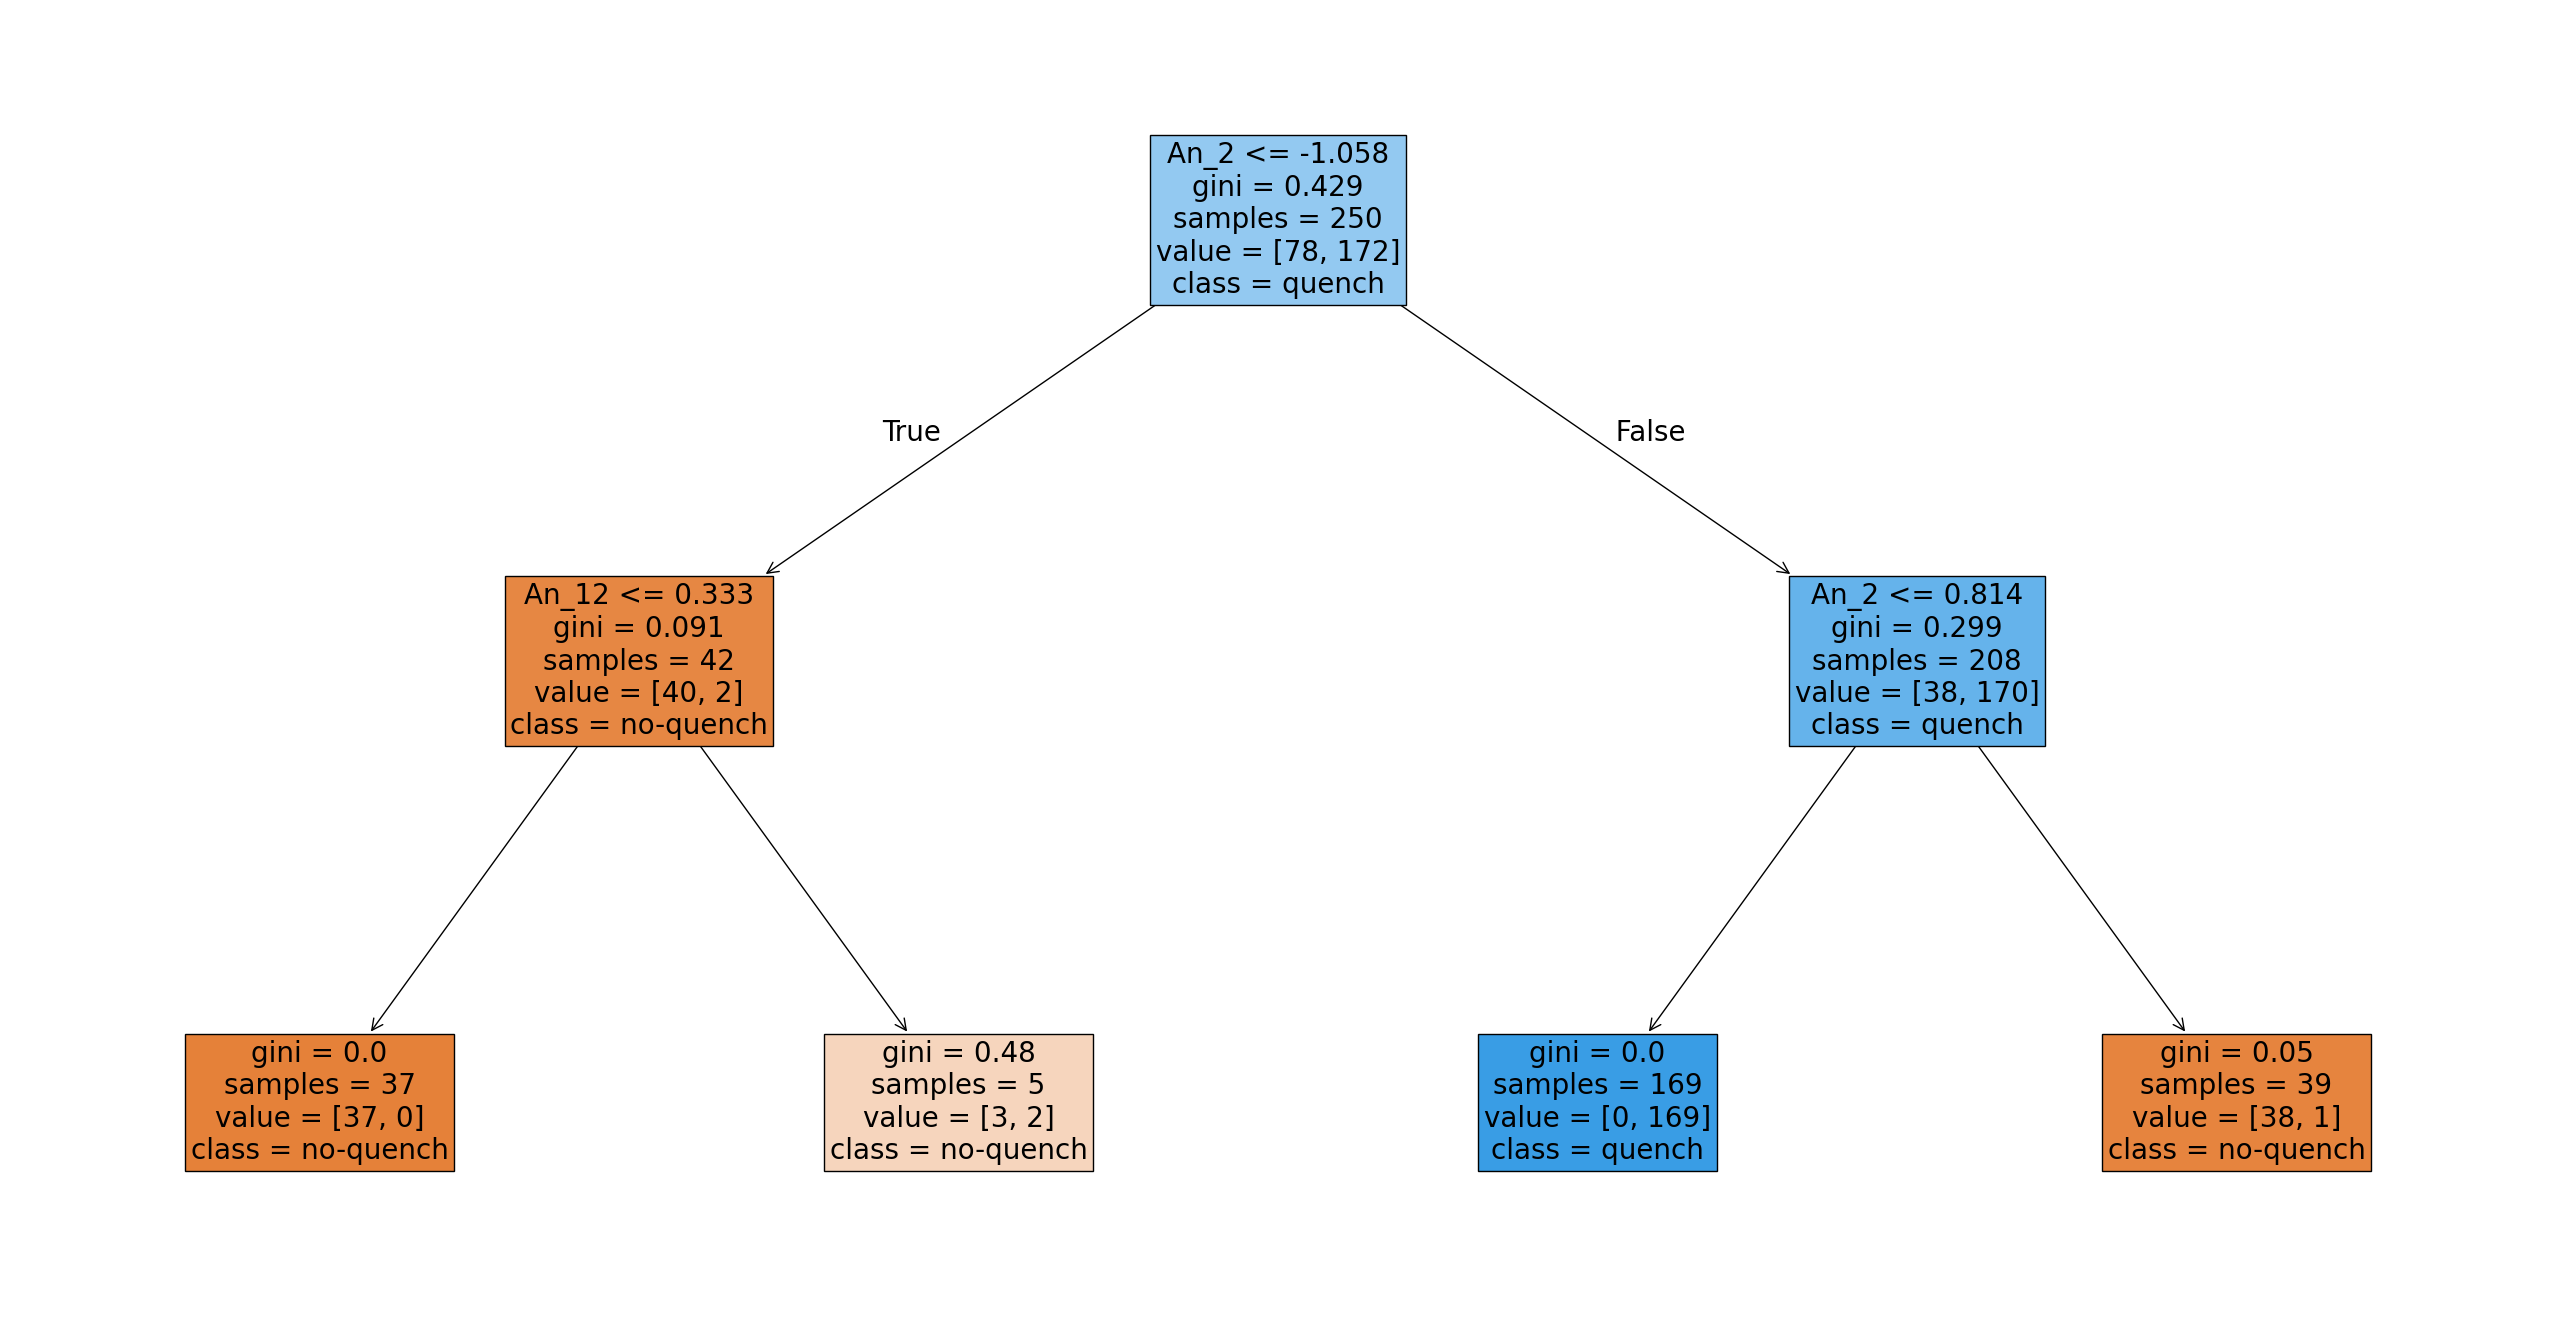
\includegraphics[width=\linewidth]{img/An_2_12_pt_dt.png}
	\caption{The structure of the tree built on harmonics $2, 12, 15$} \label{fig:dt-an-2-12-pt}
\end{figure}
All other \dts\ tested fell short of the model based on \an\ that was just described, in
\Cref{fig:best-dts} we can see a comparison of the best \dts\ built on every table, despite \cnmod\
having accuracy closer to the one obtained by the best model, it cannot recognize non-quench events
as effectively (the Irec score is lower).
\begin{figure}[t]
	\centering
	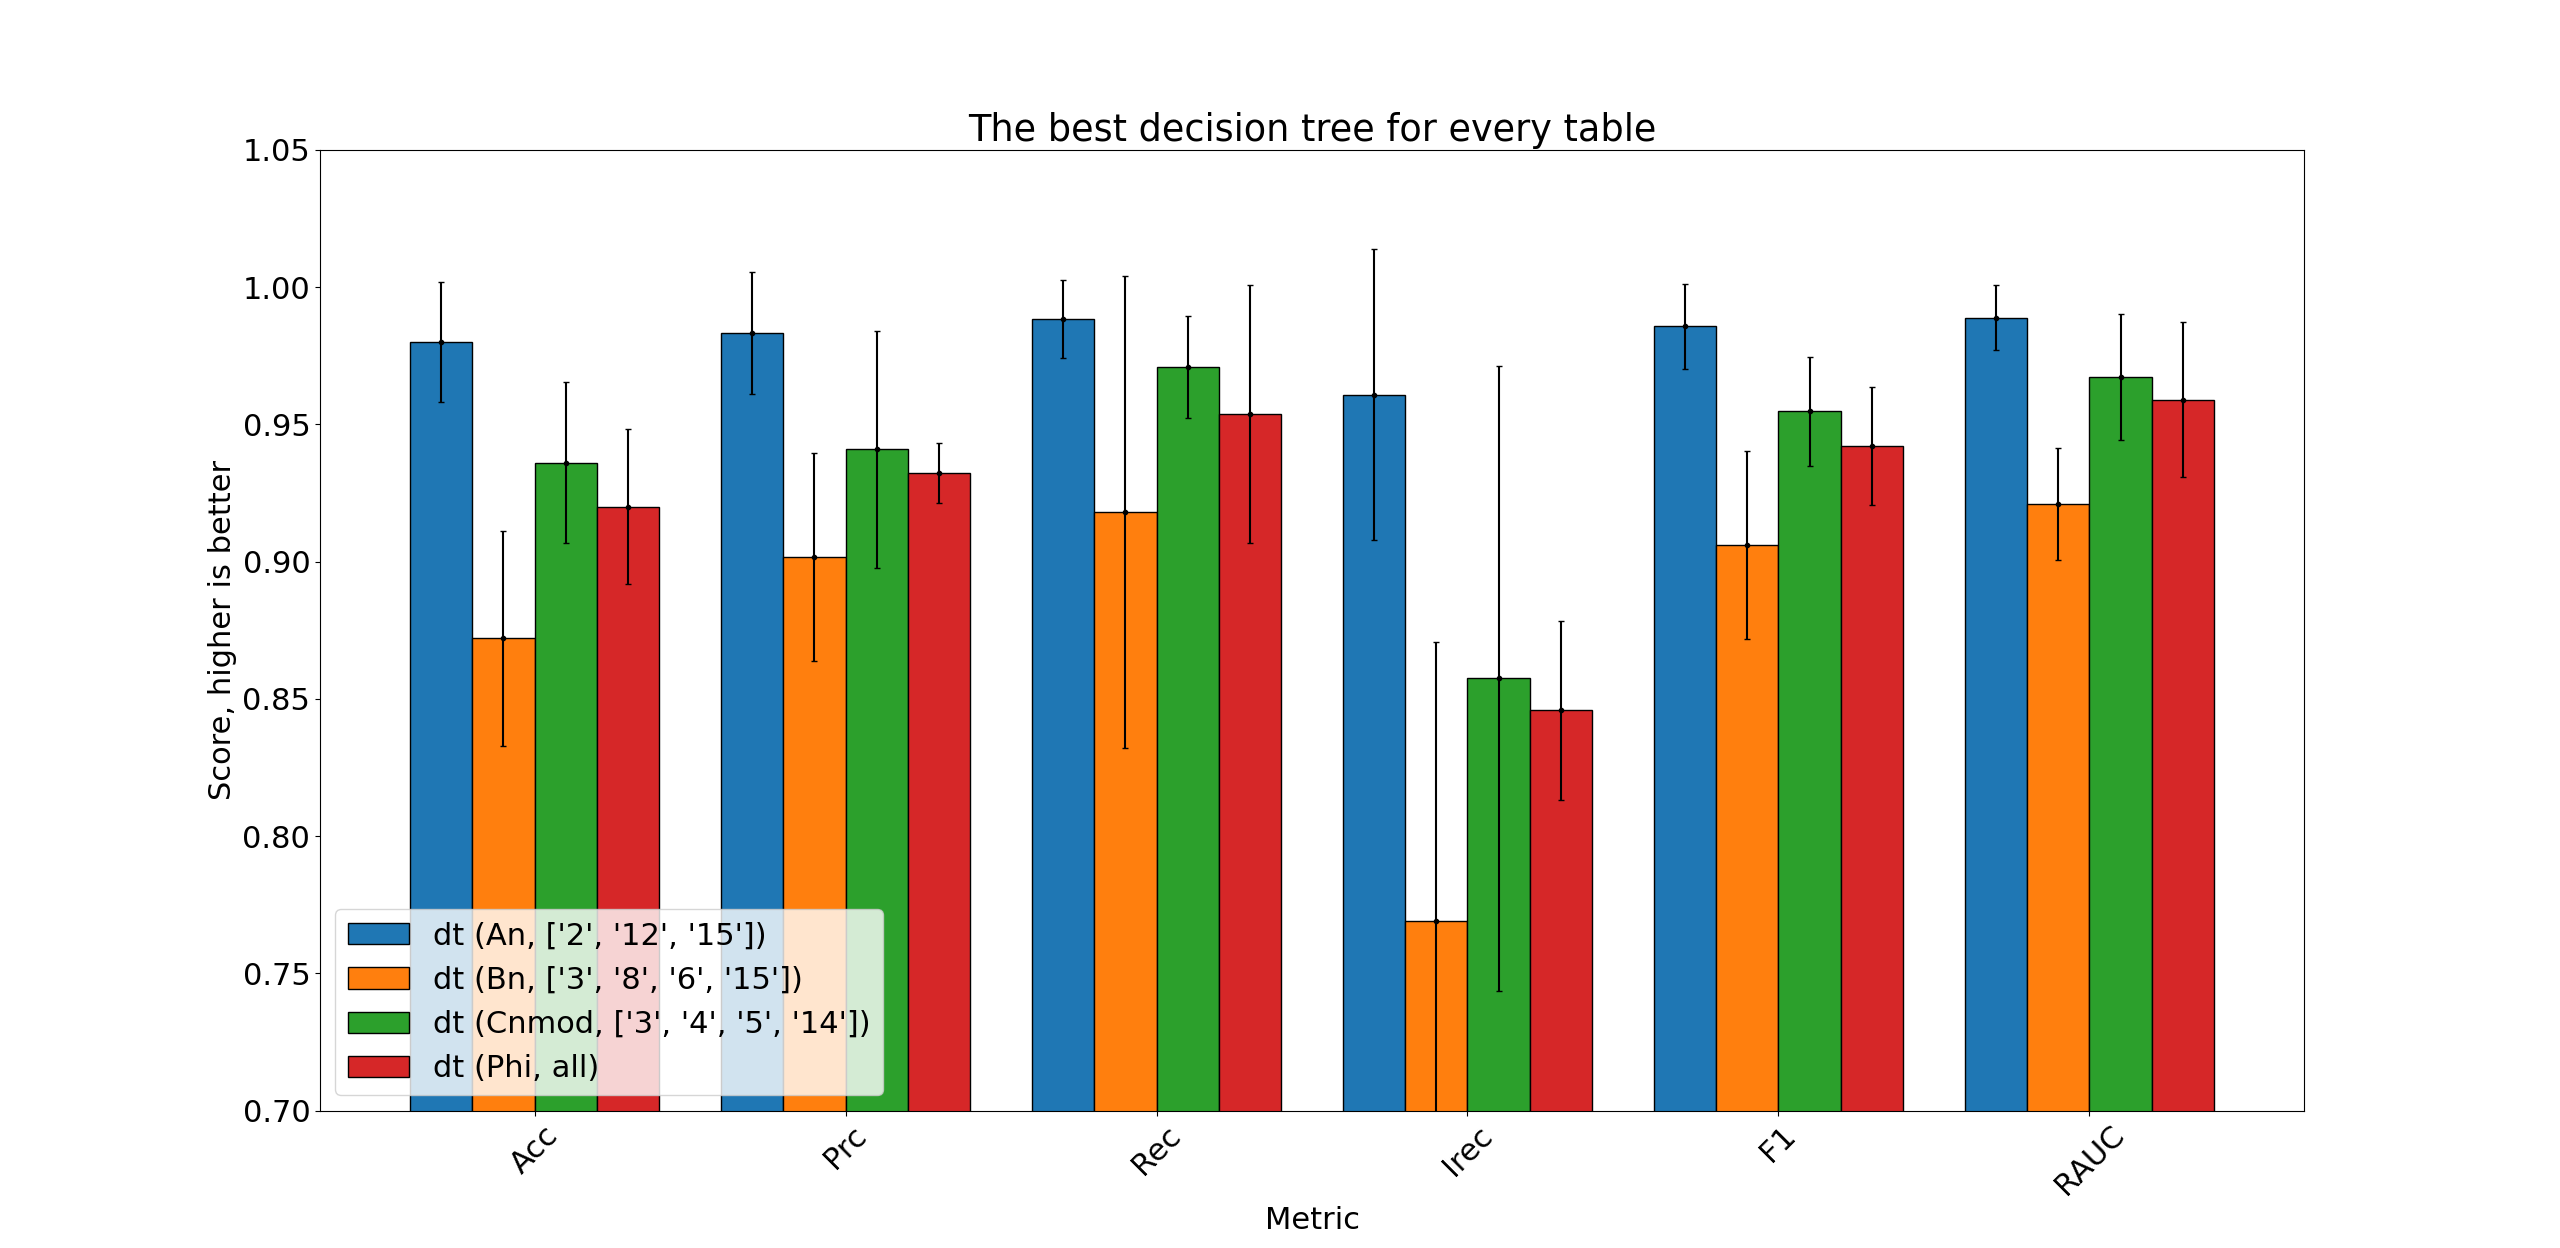
\includegraphics[width=\linewidth]{img/best_dts.png}
	\caption{Performance comparison of all the best decision trees} \label{fig:best-dts}
\end{figure}

\subsection{Random Forests}
As we said in \Cref{chp:ml} random forests (\rfs) use an ensemble of trees trained by bootstrap
sampling and perform splits on a random subset of features. As long as the trees are not too
complicated and the ensemble is not too big, \rfs\ are still quite easy to interpret, while
performing usually at least as good, if not better than the trees within the ensemble. Since \rfs\
group trees, they can easily extrapolate information from complicated datasets based on different
tables (e.g., \an, \bn, \cnmod).

In most of our tests we considered \rfs\ trained on datasets built from one or more tables, each
table taken with the full harmonic content, we also did some tests on forests built on dataset
containing a subset of the available harmonics, just we did with trees. While the second approach
was more suitable for raw performance, the first one gave us insights, through the feature
importance metric, of which were the more important harmonics within the dataset.

By analyzing the feature importance for every dataset separately and then all of them together we
can conclude the following:
\begin{itemize}
	\item The forest built on \an, performs most of the splits ($\approx 80\%$) using harmonic
	      number $2$.
	\item The forest built on \bn, performs most of the splits using a mix of different
	      harmonics, interestingly $2$ is not among the first $6$ for importance. Harmonics
	      $6, 9, 3, 14, 7$ and $5$ are the ones used the most to perform splits inside the
	      random forest.
	\item The forest built on \cnmod, uses harmonic number $2$ to perform over $50\%$ of the
	      splits, the rest are handled mainly by harmonics $5, 9$ and $13$.
	\item The forest built on \phin, uses many different harmonics to perform the splits (mainly
	      $10, 12, 6$ and $10$).
\end{itemize}
Finally, if we use the algorithm on a dataset constructed on all the tables, we can see that circa
$90\%$ of the splits were computed by using harmonics $2$ and $3$ from \cnmod, and harmonics $12, 2$
and $14$ from \an.

In \Cref{fig:best-rfs} we plotted the metrics for the $4$ best performing random forests,
independently of how they were trained, the best model achieves accuracy of $\approx 98.8\%$, while
the other models remain above $98\%$.
\begin{figure}
	\centering
	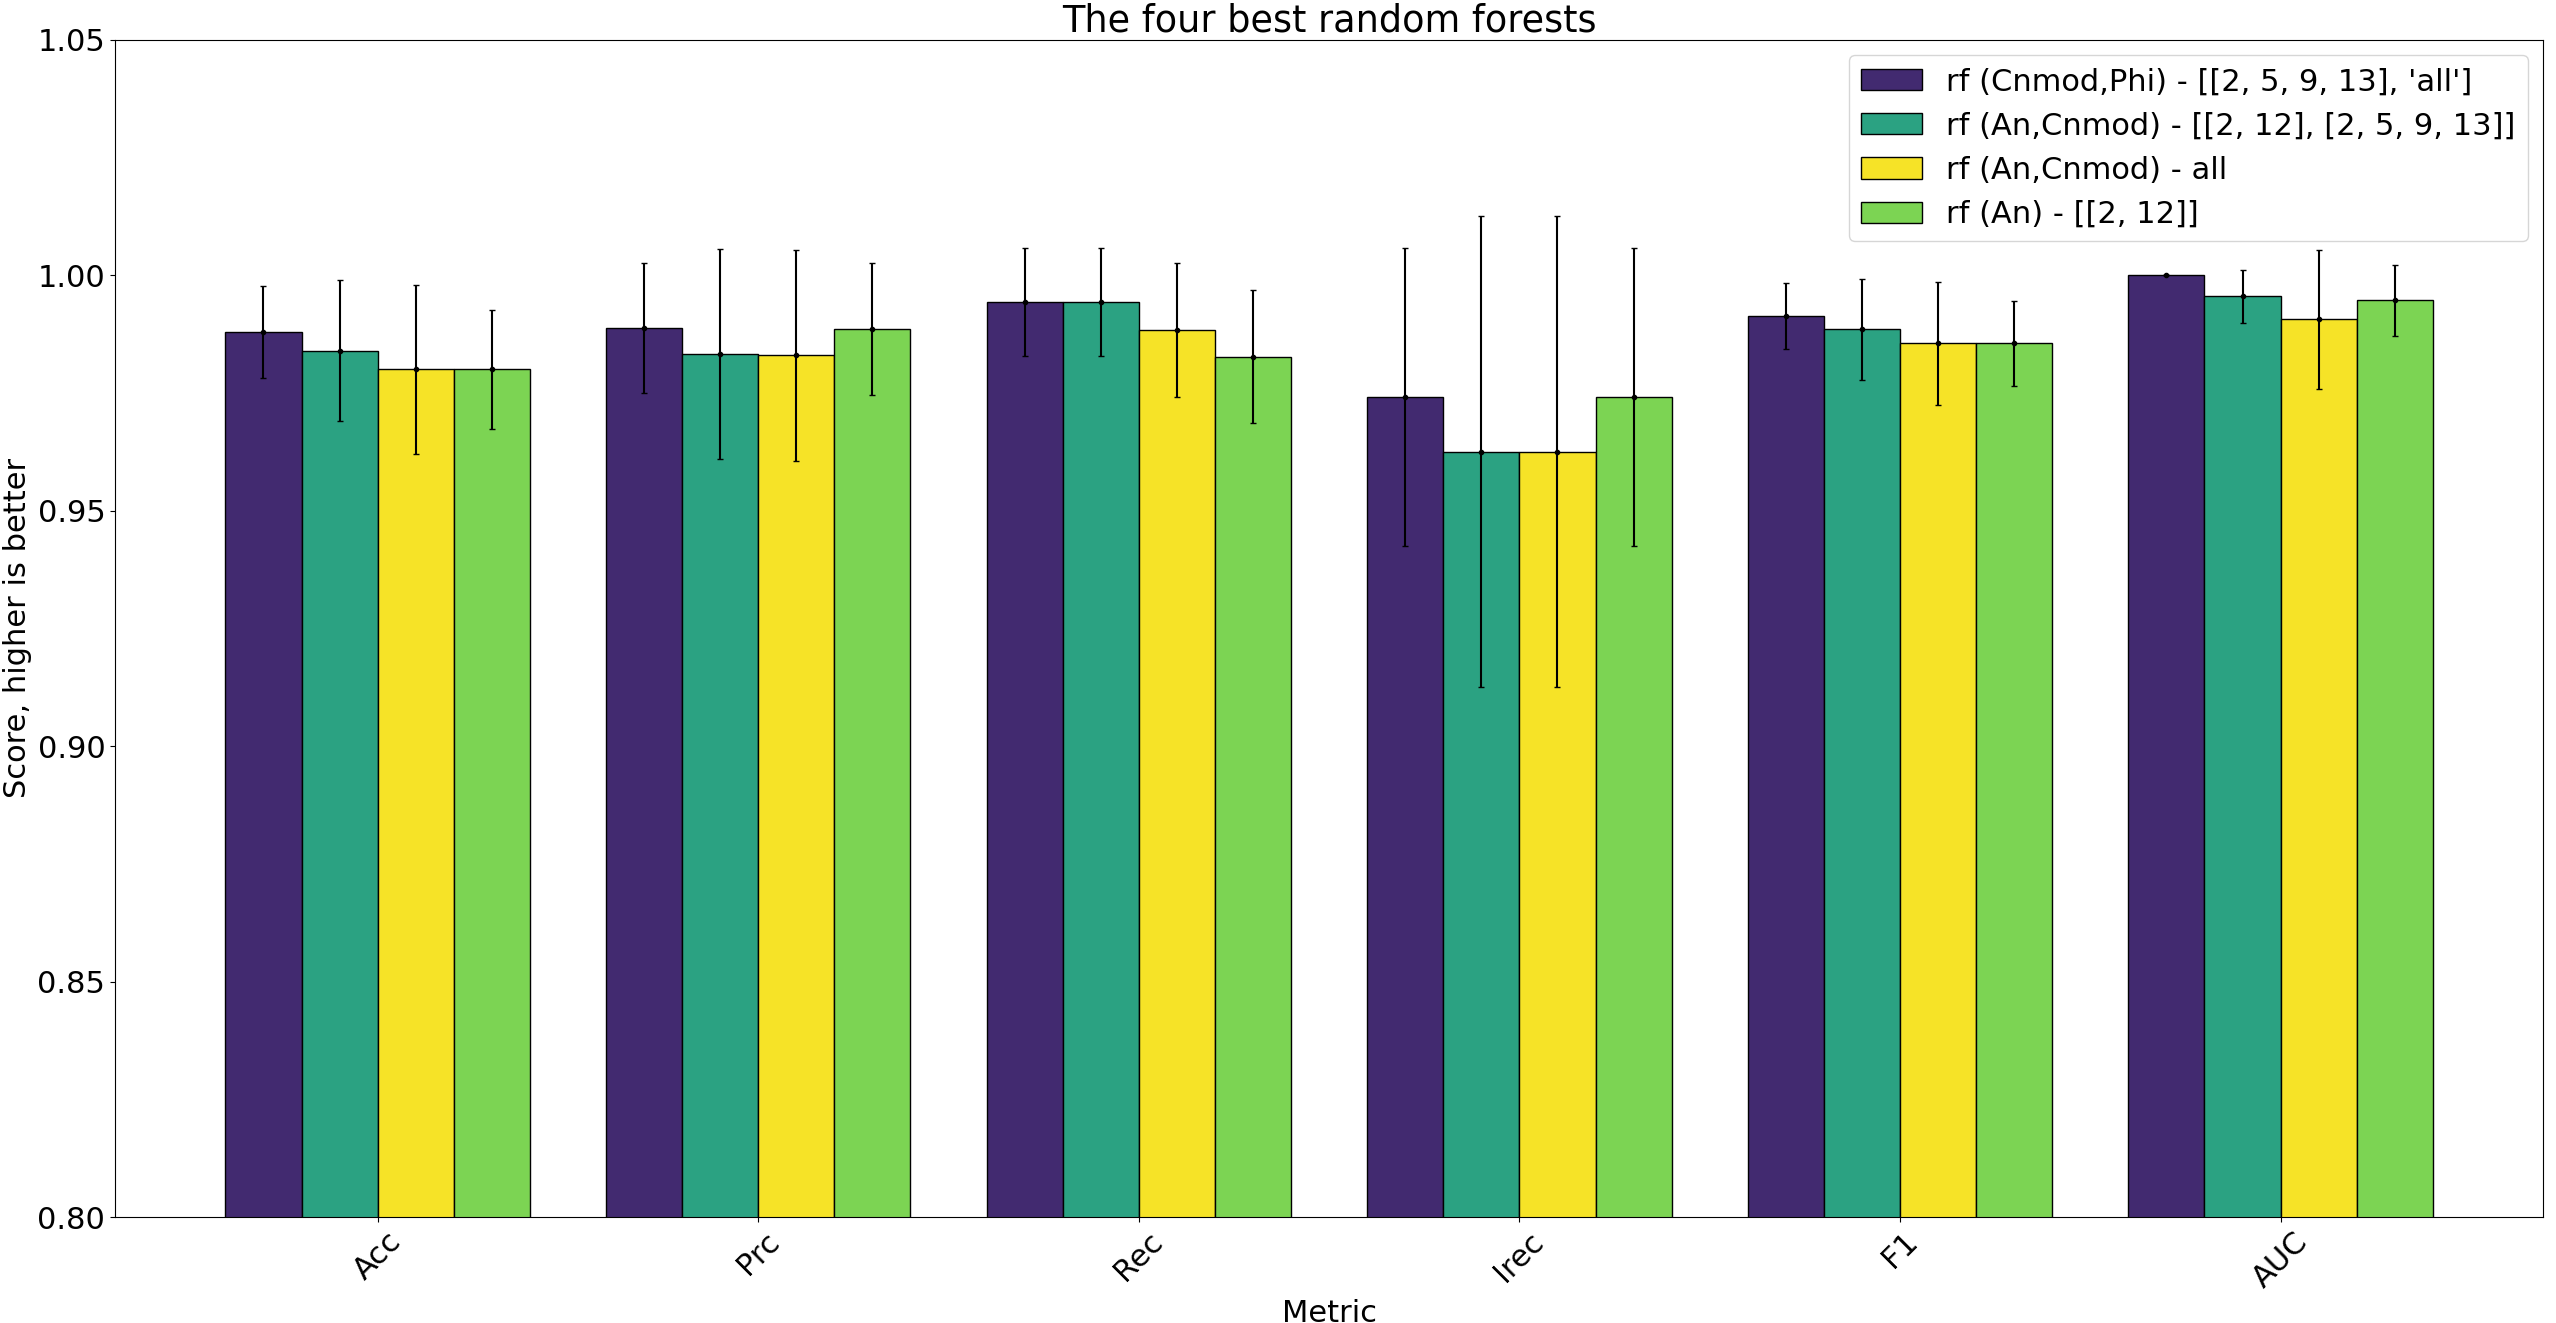
\includegraphics[width=\linewidth]{img/best_rfs.png}
	\caption{The best random forests} \label{fig:best-rfs}
\end{figure}
The performance are almost optimal, and with some more work we could probably achieve better
results, since the models considered above are trained on datasets obtained by putting together the
harmonics that perform the best for every table. This means that we are not aware if there is
strong correlation among harmonics taken from different tables.

Before concluding the section we can dedicate a table, as we did for \dts\, to the best \rf\ we
found. As we can see in \Cref{tbl:rf-cnmod-phi-perf}, the results are not too far from what we obtained with
the \dt\ in particular the random forest is considered a 'better classifier'(Since the RAUC score is
higher), having slightly better accuracy and recall while being less effective at recognizing
non-quench events, due to a lower inverse-recall score.
\begin{table}[t]
	\caption{Average and standard deviation of the performance for the best \rf\ over the outer \cv\
		folds.}\label{tbl:rf-cnmod-phi-perf}

	\bigskip
	\setlength{\tabcolsep}{6pt}
	\centering
	\begin{tabular}{ccccccc}
		\toprule
		\textbf{}    & \textbf{Acc} & \textbf{Prc} & \textbf{Rec} & \textbf{Irec} & \textbf{F1} & \textbf{RAUC} \\
		\midrule
		Mean         & 0.989        & 0.989        & 0.994        & 0.974         & 0.991
		             & 1.0                                                                                      \\
		\textsc{std} & 0.010        & 0.013        & 0.011        & 0.032         & 0.007
		             & 0.0                                                                                      \\
		\bottomrule
	\end{tabular}
\end{table}

Satisfied with the results obtained on the model, we decided to move away from \rfs to explore a new
model which has a simpler structure.

\subsection{Tree Aggregators}


%\subsection{SVM}
%Before moving onward to the other models let's consider the $\svm$, as we said in \Cref{sec:svm}, it
%is a very high performance model, capable of finding the solution with a very high accuracy. All of
%this is done my transposing the samples to a higher dimensional space where a dividing hyperplane
%can be found. Since this mapping is unknown and we are using an approximation for it, the $\svm$
%model has a very low degree of explainability.
%
%The reason why we are introducing the $\svm$ model first is because we got very high performance out
%of decision trees already, therefore we asked ourselves what was the best performance we could be
%pushing for. If we compare the best $\svm$ with the best decision tree, like we did in
%\Cref{fig:svm-vs-dt}, it's clear that there is still quite a bit of room for improvement, especially in the Inverse recall metric, which is the one where most models are at fault.
%\begin{figure}[h!]
%	\centering
%	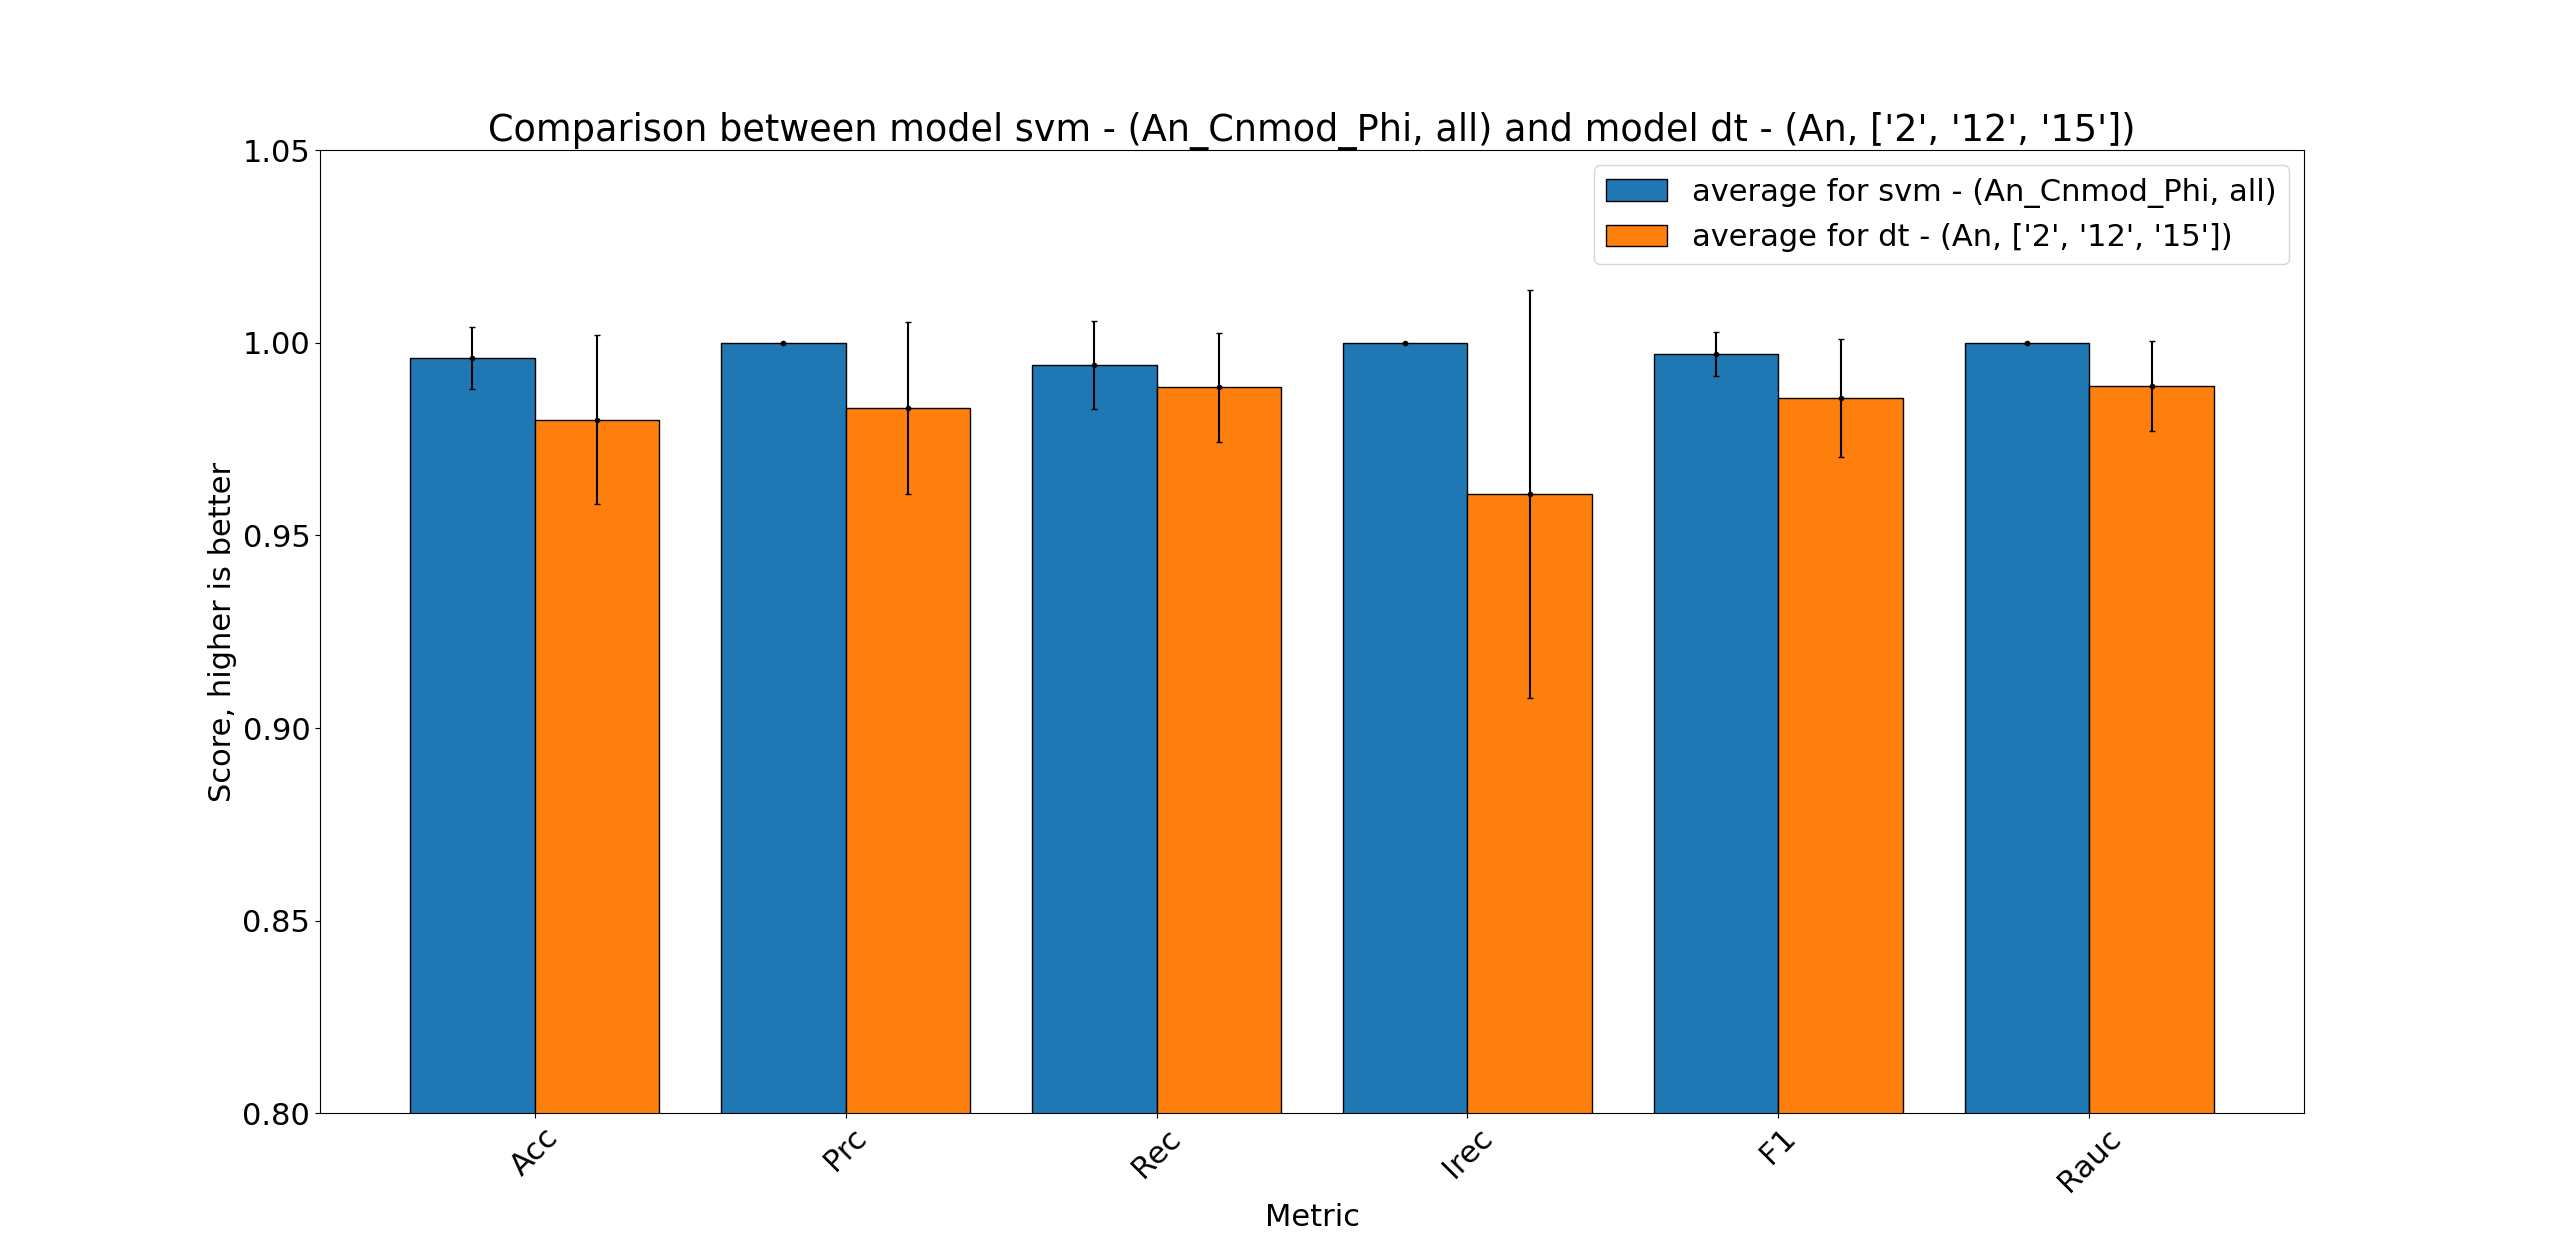
\includegraphics[width=\linewidth]{img/svm_vs_dt.png}
%	\caption{Performance comparison of $\svm$ and decision tree} \label{fig:svm-vs-dt}
%\end{figure}
%The model that are shown in this plot are:
%\begin{itemize}
%	\item The decision tree we just introduced (\Cref{fig:dt-an-2-12-15-pt}),
%	\item The $\svm$ is built on top of a mix of tables (\an, \cnmod and \phin), using the full
%	      harmonic content, a polynomial kernel of degree $3$, with a regularization parameter
%	      of $0.1$ and a kernel coefficient $\gamma = 0.1$ and a $c_0 = 0.1$. Both of these
%	      hyperparameters were not introduced in \Cref{sec:svm} because they are
%	      implementation specific, as a matter of fact, the polynomial kernel has the
%	      following structure $\kappa(x, y) = (\gamma\trans{\vec{x}}y + c_0)^d$.
%\end{itemize}
%
%In the following we will be showing two different techniques, still based on trees, which yielded
%very high performance and we will later close the chapter with an analysis of the model that we
%chose to solve the problem performed the best overall.


\subsection{Tree Aggregators}

\subsubsection{Performance on the triplets}
